% This file was converted to LaTeX by Writer2LaTeX ver. 1.2
% see http://writer2latex.sourceforge.net for more info
\documentclass[letterpaper]{article}
\usepackage[ascii]{inputenc}
\usepackage[T1]{fontenc}
\usepackage[english]{babel}
\usepackage{amsmath}
\usepackage{amssymb,amsfonts,textcomp}
\usepackage{color}
\usepackage{array}
\usepackage{supertabular}
\usepackage{hhline}
\usepackage{hyperref}
\hypersetup{pdftex, colorlinks=true, linkcolor=blue, citecolor=blue, filecolor=blue, urlcolor=blue, pdftitle=Programming Language Support for Exploratory Graphics Applicati, pdfauthor=, pdfsubject=, pdfkeywords=}
\usepackage[pdftex]{graphicx}
%\newcommand\textsubscript[1]{\ensuremath{{}_{\text{#1}}}}
% Text styles
\newcommand\textstyleHeadingivChar[1]{\foreignlanguage{english}{#1}}
% Outline numbering
\setcounter{secnumdepth}{0}
\makeatletter
\newcommand\arraybslash{\let\\\@arraycr}
\makeatother
% List styles
\newcommand\liststyleWWviiiNumv{%
\renewcommand\theenumi{\arabic{enumi}}
\renewcommand\theenumii{\arabic{enumii}}
\renewcommand\theenumiii{\arabic{enumiii}}
\renewcommand\labelitemi{[F0B7?]}
\renewcommand\labelenumi{\theenumi.}
\renewcommand\labelenumii{\theenumii.}
\renewcommand\labelenumiii{\theenumiii.}
}
\newcommand\liststyleLix{%
\renewcommand\theenumi{\arabic{enumi}}
\renewcommand\theenumii{\arabic{enumii}}
\renewcommand\theenumiii{\arabic{enumiii}}
\renewcommand\theenumiv{\arabic{enumiv}}
\renewcommand\labelenumi{\theenumi.}
\renewcommand\labelenumii{\theenumii.}
\renewcommand\labelenumiii{\theenumiii.}
\renewcommand\labelenumiv{\theenumiv.}
}
% Page layout (geometry)
\setlength\voffset{-1in}
\setlength\hoffset{-1in}
\setlength\topmargin{1in}
\setlength\oddsidemargin{1.25in}
\setlength\textheight{8.999933in}
\setlength\textwidth{6.0in}
\setlength\footskip{36.5448pt}
\setlength\headheight{0cm}
\setlength\headsep{0cm}
% Footnote rule
\setlength{\skip\footins}{0.0469in}
\renewcommand\footnoterule{\vspace*{-0.0071in}\setlength\leftskip{0pt}\setlength\rightskip{0pt plus 1fil}\noindent\textcolor{black}{\rule{0.25\columnwidth}{0.0071in}}\vspace*{0.0398in}}
% Pages styles
\makeatletter
\newcommand\ps@Standard{
  \renewcommand\@oddhead{}
  \renewcommand\@evenhead{}
  \renewcommand\@oddfoot{}
  \renewcommand\@evenfoot{}
  \renewcommand\thepage{\arabic{page}}
}
\newcommand\ps@Nextconverti{
  \renewcommand\@oddhead{}
  \renewcommand\@evenhead{}
  \renewcommand\@oddfoot{\hfill\thepage\hfill}
  \renewcommand\@evenfoot{\@oddfoot}
  \renewcommand\thepage{\arabic{page}}
}
\makeatother
\pagestyle{Nextconverti}
\thispagestyle{Standard}
\setlength\tabcolsep{1mm}
\renewcommand\arraystretch{1.3}
\title{Unicon 3D Graphics User's Guide and Reference Manual}
\author{Naomi Martinez, Clinton Jeffery, and Jafar Al Gharaibeh}
\date{2014-02-16}
\begin{document}
\clearpage\setcounter{page}{1}\pagestyle{Nextconverti}
\thispagestyle{Standard}

\ \\
\ \\
\ \\
\ \\
\ \\
\ \\
\ \\

\begin{center}
{\Large\bfseries
Unicon 3D Graphics\\
User's Guide and Reference Manual
}
\end{center}

\bigskip

\bigskip

\bigskip

\bigskip

\bigskip

\bigskip

\bigskip


{\centering\selectlanguage{english}
Naomi Martinez, Clinton Jeffery, and Jafar Al Gharaibeh
\par}

{\centering\selectlanguage{english}
Unicon Technical Report \#9d
\par}

{\centering\selectlanguage{english}
April 3, 2016
\par}

\bigskip

\bigskip

\bigskip

\bigskip

\bigskip

{\centering\selectlanguage{english}\bfseries
Abstract
\par}


\bigskip

{\selectlanguage{english}
Version 12 of the Unicon language includes 3D graphics facilities.
This document describes the design of the Unicon 3D
graphics facilities, and provides several examples detailing their use.}


\bigskip


\bigskip


\bigskip


\bigskip


\bigskip

{\centering\selectlanguage{english}
University of Idaho\\
Moscow, ID 83844
\par}

\ \\

\bigskip

\bigskip

\bigskip

\bigskip

\bigskip

\bigskip

{\selectlanguage{english}
This work was sponsored by the National Library of Medicine, the
Alliance for Minority\\ Participation, and by NSF grants
EIA-0220590 and EIA-9810732.}

\pagebreak

\section[1. Introduction]{1. Introduction}

\bigskip

Most application programming interfaces for writing 3D computer
graphics applications are complicated and difficult to
master. Toolkits such as OpenGL [OpenGL00] and Open Inventor are
powerful, but several weeks or even months are needed to gain
proficiency. Even after gaining proficiency, many lines of code are
required to implement most features. There is much that can be
simplified.

Unicon [Jeffery03] is a superset of the Icon programming language
[Griswold96] that offers many features that minimize the time and
effort spent programming. Programs written in Unicon require from two
to ten times fewer lines of code than programs written in languages
such as C, C++, or Java. This report describes a set of simple, easy
to use 3D graphics facilities for Unicon.

Icon and Unicon already provide facilities that simplify the process
of programming 2D graphics applications [Griswold98]. Unicon's 3D
graphics facilities are based upon and integrated with the 2D
facilities. Unicon's 3D facilities are built on top of one of the
leading 3D graphics libraries, OpenGL. OpenGL is more widely portable
and available than most similar toolkits.

This paper discusses the design and demonstrates the use of Unicon's
3D graphics facilities. Section two contains the design of the Unicon
3D graphics facilities. Examples and sample code can be found in
section three. References for functions and attributes are found in
section four. The implementation of the Unicon 3D graphics facilities
is discussed in [JeffMart03].


\section[2. Design]{2. Design}


The Unicon 3D graphics facilities aim to provide the basic elements of
3D computer graphics in a simplified fashion. The basic functionality
includes primitives, transformations, lighting, and texturing. With
these features, the Unicon 3D graphics facilities should provide a
good basis to construct an OpenGL scene using Unicon.

The features of the Unicon 3D graphics facilities differ from the
features of OpenGL in several ways. The Unicon 3D graphics facilities
introduce several not available in OpenGL. These features include the
direct use of image files as textures and the use of the foreground
attribute to manipulate material properties. Also there are several
features of OpenGL that are not available in the Unicon 3D graphics
facilities. These feature include blending, fog, antialiasing, display
lists, selection, and feedback. If there is need to, future work might
include implementing these features.

\subsection[2.1 Application Programming Interface (API)
Reduction]{\bfseries 2.1 Application Programming Interface (API) Reduction}

OpenGL contains over 250 functions that can be called to render 3D
graphics applications. Also needed are many window system calls that
are not provided by OpenGL, to open and close windows and handle input
from the user. The Unicon 3D graphic facilities reduce the number of
functions that a Unicon user must typically learn to use. The Unicon
3D graphics facilities contain sixteen new functions and six functions
that have been extended from the 2D graphics facilities.

Some of the API reduction was obtained by trivial application of
Unicon language features. The ability to store different data types in
the same variable and the fact that Unicon handles functions with a
variable number of arguments and varying types reduced the number of
functions needed in the API. For example there are six different
functions one can call to clear a window in OpenGL. Unicon users only
need one. Other methods of reduction include providing OpenGL features
with default parameters and eliminating unnecessary function calls.


\subsection[2.2 Opening Windows for 3D Graphics]
{2.2 Opening Windows for 3D Graphics}


The first step in 3D graphics programming is opening windows to render
3D graphics, as in the line:

{\sffamily
W := open(``win'', ``gl'')}


\bigskip

To open a 3D graphics window, call the built in function
\textsf{open()}, passing in the title of the window to be
opened and mode \textsf{``gl''}. In the above example,
\textsf{``win''} is the title of the window to be opened. The
parameter \textsf{``gl''} indicates that a window for rendering 3D
graphics should be opened. As in the 2D facilities, if a window is
assigned to the keyword variable \textsf{\&window}, it is a default
window for subsequent 3D function calls. The newly opened window can
be queried for the specifications of the 3D graphics library. The
following example demonstrates the use of such attributes:

\textsf{procedure main(av)}

\textsf{ \ \ \&window := open({\textquotedbl}gl attributes{\textquotedbl}, {\textquotedbl}gl{\textquotedbl},
``canvas=hidden'')}

\textsf{ \ \ write({\textquotedbl}glversion \ : {\textquotedbl},
 WAttrib({\textquotedbl}glversion{\textquotedbl}))}

\textsf{ \ \ write({\textquotedbl}glvendor \ \ : {\textquotedbl},
 WAttrib({\textquotedbl}glvendor{\textquotedbl}))}

\textsf{ \ \ write({\textquotedbl}glrenderer : {\textquotedbl},
 WAttrib({\textquotedbl}glrenderer{\textquotedbl}))}

\textsf{end}

\noindent
and here is a sample output of the program after running it on
some specific hardware:\newline
\newline
\textsf{glversion \ : 2.1.2 NVIDIA 195.36.15\newline
glvendor \ \ : NVIDIA Corporation\newline
glrenderer : Quadro FX Go1400/PCI/SSE2}\newline


\subsection[2.3 The Coordinate System]{2.3 The Coordinate System}

Features such as lighting, perspective, texturing, and shading, give
a scene the illusion of being three-dimensional. In order to control
such features, a Unicon programmer makes use of context attributes.
By assigning new values to various attributes the programmer can
effectively change many aspects of the scene. Attributes to control
the coordinate system, field of view, lighting and textures are
included in the Unicon 3D graphics facilities.

Some of the most basic context attributes concern the coordinate
system. In 3D graphics one can think of drawing the scene in a
three-dimensional coordinate system. A set of three numbers, an
x-coordinate, a y-coordinate, and a z-coordinate, determine where to
place an object. The objects that are visible on the screen depend on
several things, the eye position, the eye direction, and the
orientation of the scene. If these things are not taken into account,
the scene drawn and the scene desired by the user might be two very
different things.

To help think about these attributes, imagine a person walking around
a 3D coordinate system. What this person sees becomes the scene viewed
on the screen. The eye position specifies where this person is
standing. For instance if this person is standing at the origin,
\textsf{(0, 0, 0),} then things close to the origin appear larger and
seem closer than objects further from the origin. The eye direction
supplies the direction in which the person is looking. Suppose the
person is looking toward the negative z-axis. Then only the objects
situated on the negative z-axis are viewed in the scene. Anything on
the positive z-axis is behind the viewer. Finally, the up direction
can be described by what direction is up for the person.

In the Unicon 3D graphics facilities, the eye position is given by the
attribute \textsf{eyepos}. By default this is set to be at the origin
or \textsf{(0, 0, 0)}. The eye direction is given by the attribute
\textsf{eyedir}. By default this is set to be looking at the negative
z-axis. The up direction can be specified by the attribute
\textsf{eyeup} and by default is \textsf{(0, 1, 0)}. The attribute
\textsf{eye} allows the user to specify \textsf{eyepos},
\textsf{eyedir}, and \textsf{eyeup} with a single value; for
convenience a function \textsf{Eye()} sets these attributes directly
from numeric parameters. After changing any of these attributes, the
scene will redraw itself with the new eye specifications.


\bigskip

\subsection[2.4 Drawing Primitives]{2.4 Drawing Primitives}

In the Unicon 2D graphics facilities, a user can draw 2D points,
lines, polygons, and circles. Primitives analogous to these and more
are available in Unicon's 3D graphics facilities. The Unicon 3D
primitives are a cube, a point, a line, a line segment, a sphere, a
torus, a cylinder, a disk, a partial disk, a filled polygon, and an
outline of a polygon.  These are described in Table 1 below. All
functions specified, can take as their first parameter the window to
be drawn on. When a window is not specified the primitives will be
drawn on the default window, \textsf{\&window}.

In the Unicon 3D graphics facilities, one can draw 2D, 3D or 4D
objects within the same scene. With the use of the context attribute,
\textsf{dim}, the user can switch between the different dimensions of
an object. A user can draw 2D, 3D, or 4D, objects by assigning
\textsf{dim} the values of 2, 3, or 4. It is worth noting that a 2D
object drawn in a 3D scene does not use Unicon's 2D graphics
facilities for its implementation. Instead, the \textsf{dim}
attribute defines how many components a vertex of a primitive will
have. The value of \textsf{dim} affects the primitives drawn in
several ways. For functions such as \textsf{DrawPolygon()} which take
the coordinates of each vertex as parameters, the value of
\textsf{dim} specifies the number of parameters each vertex will
have. For primitives that take x, y, and z coordinates, specifying
only x and y coordinate is not sufficient. For this reason,
\textsf{{}``dim = 2''} disallows the use of these primitives. These
functions are
\textsf{DrawSphere(), DrawTorus(), DrawCube(), and DrawCylinder()}.
By default the value of \textsf{dim} is
three. An example of drawing primitive can be found in section 3.2.


\bigskip

{\centering\selectlanguage{english}\bfseries
Table 1 -- types of primitives
\par}

\begin{center}
\tablefirsthead{}
\tablehead{}
\tabletail{}
\tablelasttail{}
\begin{supertabular}{|m{0.89835984in}|m{1.3677598in}|m{2.2177598in}|m{1.1962599in}|}
\hline
\centering{\selectlanguage{english} Primitive} &
\centering{\selectlanguage{english} Function} &
\centering{\selectlanguage{english} Parameters} &
\centering\arraybslash{\selectlanguage{english} Picture}\\\hline
{\selectlanguage{english} Cube} &
{\selectlanguage{english}\sffamily DrawCube()} &
{\selectlanguage{english} the x, y, and z coordinates of the lower left front corner, and the length of the sides. } &
\centering\arraybslash  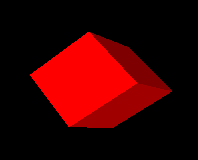
\includegraphics[width=0.9543in,height=0.772in]{utr9/utr9-img001.png} \\\hline
{\selectlanguage{english} Cylinder} &
{\selectlanguage{english}\sffamily DrawCylinder()} &
{\selectlanguage{english} the x, y, and z coordinates of the center, the height, the radius of the top, the radius of
the bottom. If one radius is smaller than the other a cone is formed. } &
{\centering  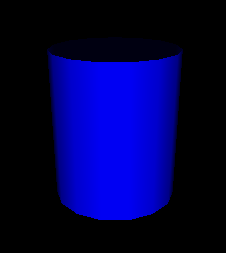
\includegraphics[width=0.798in,height=0.7035in]{utr9/utr9-img002.png} \par}
\centering\arraybslash  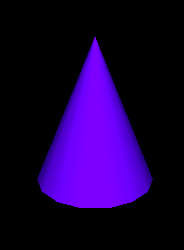
\includegraphics[width=0.7965in,height=0.8772in]{utr9/utr9-img003.png} \\\hline
{\selectlanguage{english} Disk} &
{\selectlanguage{english}\sffamily DrawDisk()} &
{\selectlanguage{english} the x, y, and z coordinates of center, the radius of the inner circle, and the radius of the
outer circle. By specifying an additional two angle values a partial disk is obtained. } &
{\centering  
\includegraphics[width=0.8992in,height=0.7571in]{utr9/utr9-img004.png} \par}
\centering\arraybslash  
\includegraphics[width=0.8992in,height=0.7598in]{utr9/utr9-img005.png} \\\hline
{\selectlanguage{english} Filled Polygon} &
{\selectlanguage{english}\sffamily FillPolygon()} &
{\selectlanguage{english} the x, y, and z coordinates of each vertex of the polygon. } &
\centering\arraybslash  
\includegraphics[width=0.9429in,height=0.6217in]{utr9/utr9-img006.png} \\\hline
{\selectlanguage{english} Line} &
{\selectlanguage{english}\sffamily DrawLine()} &
{\selectlanguage{english} the x, y, and z coordinates of each vertex of the line. } &
\centering\arraybslash  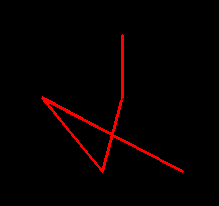
\includegraphics[width=0.9417in,height=0.5957in]{utr9/utr9-img007.png} \\\hline
{\selectlanguage{english} Polygon} &
{\selectlanguage{english}\sffamily DrawPolygon()} &
{\selectlanguage{english} the x, y, and z coordinates of each vertex of the polygon. } &
\centering\arraybslash  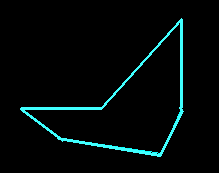
\includegraphics[width=0.9417in,height=0.6043in]{utr9/utr9-img008.png} \\\hline
{\selectlanguage{english} Point} &
{\selectlanguage{english}\sffamily DrawPoint()} &
{\selectlanguage{english} the x, y, and z coordinates of each individual point.} &
\centering\arraybslash  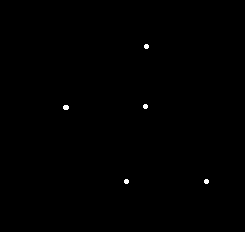
\includegraphics[width=0.9429in,height=0.5957in]{utr9/utr9-img009.png} \\\hline
{\selectlanguage{english} Segment} &
{\selectlanguage{english}\sffamily DrawSegment()} &
{\selectlanguage{english} the x, y, and z coordinates of each vertex of the line segments.} &
\centering\arraybslash  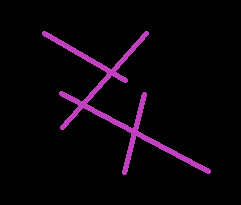
\includegraphics[width=0.9362in,height=0.6425in]{utr9/utr9-img010.png} \\\hline
{\selectlanguage{english} Sphere} &
{\selectlanguage{english}\sffamily DrawSphere()} &
{\selectlanguage{english} the x, y, and z coordinates of center and the radius of the sphere. } &
\centering\arraybslash  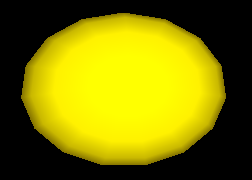
\includegraphics[width=0.9307in,height=0.6543in]{utr9/utr9-img011.png} \\\hline
{\selectlanguage{english} Torus} &
{\selectlanguage{english}\sffamily DrawTorus()} &
{\selectlanguage{english} the x, y, and z coordinates of the center, an inner radius and an outer radius. } &
\centering\arraybslash  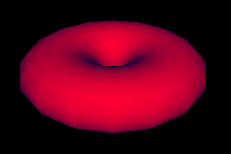
\includegraphics[width=0.9398in,height=0.6272in]{utr9/utr9-img012.png} \\\hline
\end{supertabular}
\end{center}

Several functions from the 2D graphics facilities have been extended
for the 3D graphics facilities. By doing this, learning to use the
Unicon 3D graphics facilities may be easier for users of the Unicon 2D
graphics facilities. These functions are
\textsf{DrawPoint(), DrawLine(), DrawSegment(), DrawPolygon()} and
\textsf{FillPolygon()}, which
draw a point, a line, a line segment, an outline polygon or a filled
polygon, respectively. Through the use of the already present 2D
functions, the number of functions added for the 3D graphics
facilities are kept to a minimum.



\subsection[2.5 Transformations]{2.5 Transformations}

Matrix multiplications are used to calculate transformations, such as
rotations, translations, and scaling, on objects and the field of
view. In order for the user to keep track of matrices and matrix
multiplications, functions to perform several operations are included
in Unicon's 3D graphics facilities.

In many 3D graphics applications, several transformations are
performed on one object and several other transformations are
performed on another object. For this reason, it is desirable to use
different matrices to perform these calculations. OpenGL keeps track
of the current matrix with a stack of matrices, where the top of the
stack is the current matrix. The Unicon 3D graphics facilities make
use of OpenGL's implementation of the matrix stack to implement
transformations.

Several functions are provided to the Unicon user to manipulate the
matrix stack. The function \textsf{PushMatrix()} pushes a copy of the
current matrix onto the stack. By doing this the user can compose
several different transformations. The function
\textsf{IdentityMatrix()} changes the current matrix to the identity
matrix. Finally, to discard the top matrix and to return to the
previous matrix, the function \textsf{PopMatrix()}will pop the top
matrix off the matrix stack.

As in OpenGL, there are two different matrix stacks, projection and
modelview, in the Unicon 3D graphics facilities. The projection matrix
stack contains matrices that perform calculations on the field of
view. These calculations are based on the current eye attributes. If
these eye attributes are changed, then previous manipulations of the
projection matrix stack are no longer valid. The maximum depth of the
projection matrix stack is two. Trying to push more than two matrices
onto the projection matrix stack will generate a runtime error. The
modelview matrix stack contains matrices to perform calculations on
objects within the scene. Transformations formed using the matrix
stack only effect the objects that a programmer desires. The maximum
depth of this stack is thirty-two. So, pushing more than thirty two
matrixes onto the modelview matrix stack will generate an
error. Furthermore, only one matrix stack can be manipulated at any
given time. The function \textsf{MatrixMode() }switches between the
two matrix stacks.

\subsection[2.6 Lighting and Materials]{2.6 Lighting and Materials}

The use of lighting is an important step in making a 3D graphics scene
appear to be 3D. Adding lighting to a scene can be fairly
complicated. A light source can emit different types of light: ambient
light, diffuse light, and specular light. Ambient light is light
that has been scattered so much that is difficult to determine the
source. Backlighting in a room is an example of ambient light. Diffuse
light comes from one direction. This type of light mostly defines what
color the object appears to be. Finally, specular light not only comes
from one direction, but also tends to bounce off the objects in the
scene.

Lighting has been implemented in the Unicon graphics facilities
through the use of context attributes. The use of context attributes
reduces the number of functions added to the Unicon 3D graphics
facilities. For a 3D scene implemented in Unicon, there are eight
lights available. Using the attributes \textsf{light0} through
\textsf{light7} one can control the eight lights. Each light is
\textsf{on} or \textsf{off} and has the properties \textsf{diffuse},
\textsf{ambient}, \textsf{specular}, and \textsf{position}.

A scene not only has several lighting properties, but the objects in
scene may have several material properties. The material properties
are ambient, diffuse, and specular, which are similar to the light
properties, emission, and shininess. If an object has an emission
property, it emits light of a specific color. Using combinations of
these material properties one can give an object the illusion of being
made of plastic or metal.

In the Unicon 2D graphics facilities, users use a rich naming scheme
to specify the current foreground color using the attribute
\textsf{fg}. Colors can be specified using a string name, a
hexadecimal number, or red, green, and blue components each between
\textsf{0} and \textsf{65535}. The 3D graphics facilities have
extended this idea to the lighting and material properties. For a
material property, the programmer can specify the material property by
stating the type of the material property and then the color that the
property should have. Similarly the values for each of the lights
follow the same pattern. Also, not only can a programmer specify a
color in the same ways as the 2D graphics facilities, but also a color
can be given by providing the red, green, and blue intensities between
\textsf{0.0} and \textsf{1.0}. Examples of lighting and material
properties can be found in section 3.3.

By extending the features of the 2D graphics facilities, adding and
changing properties of lights and material has been simplified.
Furthermore, the use of the foreground attribute greatly reduces
the number of lines of code needed for a scene. This design along
with several defaults, a user of the Unicon 3D graphics facilities
can have lighting in a 3D graphics application without much effort.


\subsection[2.7 Textures]{2.7 Textures}

Another important area of three-dimension computer graphics is
textures. Adding textures to a scene can give it a more realistic
feel. In order to implement textures in the Unicon 3D graphics
facilities, several aspects of texturing have to be taken into
account. A texture image can be viewed as a rectangular image that is
``glued'' onto objects in a scene. The appearances of the textured
objects in the scene depend on several key pieces of information
supplied by the programmer. These include the texture image and what
parts of the texture image are mapped to what parts of an object.

Since not all scenes require the use of textures, the attribute
\textsf{texmode} is included in the Unicon 3D graphics facilities. By
default, textures are turned off. In order to turn on texturing in a
scene use the following line of code

{\selectlanguage{english}\ttfamily
\ \ \ \textsf{WAttrib(W, ``texmode=on'')} }

Once textures are turned on and a texture image is given, the texture
image will be applied to subsequent objects in the scene. By using the
following line of code, textures will be disabled for all successive
objects.

{\selectlanguage{english}\ttfamily
\ \ \ \textsf{WAttrib(W, ``texmode=off'')}}

Texture images in OpenGL programs are images that have been encoded
into an array. So if a programmer wants to use a .gif image file, the
file must be converted into a format accepted by OpenGL. Often times
this is a cumbersome process to obtain the desired result. For this
reason, the Unicon 3D graphics facilities provide several different
formats to specify a texture image. A texture image can be another
Unicon window, an image file, or a string. If the texture image is a
string it must be encoded in one of two language standard
formats. Either it is in the format

{\selectlanguage{english}\sffamily
{}``width,pallet,data'' \ \textrm{or} \ {}`` width,\#,data''}

\noindent where \textsf{pallet} is one of the pallets described in the 2D
graphics facilities and data is a hexadecimal representation of an
image. In the first case the pallet will determine what colors appear
in the texture image. In the second case, the foreground color and
background color will be used. The ability to use another Unicon
window as a texture provides the programmer with greater flexibility
for texture images. For OpenGL, a texture image must be known before
the start of the program. The use of a window as a texture allows
the programmer to create a texture image dynamically.

On many 3D platforms,
textures must have a height of 2\textsuperscript{n} pixels and width
of 2\textsuperscript{m} pixels where n and m are integers. If not, the
texture dimensions are automatically scaled down to the closest power
of 2. Rescaling affects application performance and may cause visual
artifacts, so it is best to create textures with appropriate sizes
in the first place. Section 3.4 contains examples on how to use
textures specified in the different forms.

A programmer can give the texture in one of two ways, one can use
\textsf{WAttrib(``texture={\dots}'') }or the function
\textsf{Texture(t)}\texttt{.} These methods do differ in one important
way, a window cannot be used as a texture with \textsf{WAttrib()}. So
a function call must be made to \textsf{Texture()} if a window is to
be used as a texture.

For textures, a programmer must specify how a texture is applied to
particular object. This is done by specifying texture coordinates and
vertices. Since a texture image can be viewed as a rectangular image,
texture coordinates are x and y coordinates of the texture image. So
the texture coordinate \textsf{(0.0, 0.0)} corresponds to the lower
left hand corner of the texture image. The texture coordinates are
mapped to the vertices specified by the programmer. These vertices are
usually the vertices of an object in the scene. Together, the texture
coordinates and the vertices determine what the scene looks like after
textures have been applied.

The design of textures in the Unicon 3D graphics facilities aims to
simplify the process of mapping a texture onto an object by setting
defaults for texture coordinates. There are several ways to specify
texture coordinates. To use the defaults given by the Unicon 3D
graphics facilities, one can either use
\textsf{WAttrib(``texcoord=auto'')} or
\textsf{Texcoord(``auto'')}. The defaults are dependent on the type of
primitive and are outlined in Table 2.

If the programmer wishes to use texture coordinates other than the
defaults, these can be specified in several ways.  One can use
\textsf{WAttrib(``texcoord=s'')} where \textsf{s} is a comma separated
string of real number values between \textsf{0.0} and
\textsf{1.0}. Each pair of values is to be taken as one texture
coordinate; there must be an even number of decimal values or the
assignment of texture coordinates will fail. Also one can assign
texture coordinates by \textsf{Texcoord(x1, y1, {\dots})} where each
\textsf{x} and \textsf{y} are real number values between \textsf{0.0}
and \textsf{1.0}. Finally one can use \textsf{Texcoord(L)} where
\textsf{L} is a list of real number texture coordinates. The texture
coordinates specified by the programmer are used differently depending
on the type of primitive to be drawn. If the primitive is a point,
line, line segment, polygon, or filled polygon, then a texture
coordinate given is assigned to each vertex. If there are more texture
coordinates than vertices, the unused texture coordinates are
ignored. If there are more vertices than texture coordinates the
application of a texture will fail.  In order to use non default
texture coordinates with cubes, tori, spheres, disks, and cylinders a
programmer should approximate the desired mapping with filled
polygons. These specifications are given in the following table.

\pagebreak

{\centering\selectlanguage{english}\bfseries
Table 2 -- texture coordinates and primitives
\par}

\begin{center}
\tablefirsthead{}
\tablehead{}
\tabletail{}
\tablelasttail{}
\begin{supertabular}{|m{0.7400598in}|m{3.2761598in}|m{0.99975985in}|m{0.7483598in}|}
\hline
\centering{\selectlanguage{english}\bfseries Primitive} &
{\centering\selectlanguage{english}\bfseries Default Texture Coordinates\par}

\centering{\selectlanguage{english} (from [OpenGL00] chapter 6)} &
\centering{\selectlanguage{english}\bfseries Effect of Non-default Texture Coordinates} &
\centering\arraybslash{\selectlanguage{english}\bfseries Picture}\\\hline
{\selectlanguage{english} Cube} &
{\selectlanguage{english} The texture image is applied to each face of the cube. } &
{\selectlanguage{english} None} &
 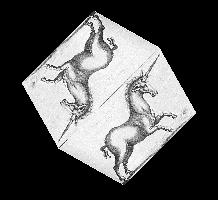
\includegraphics[width=0.728in,height=0.6689in]{utr9/utr9-img013.jpg} \\\hline
{\selectlanguage{english} Sphere}

~

~

{\selectlanguage{english} Cylinder} &
{\selectlanguage{english} The y texture coordinate ranges linearly from 0.0 to 1.0. On spheres this is from\newline
z= -radius to z=radius; on cylinders, from\newline
z = 0 to z = height. The x texture coordinate ranges from 0.0 at the positive y-axis to 0.25 at the positive x-axis,
to 0.5 at the negative\newline
y-axis to 0.75 at the negative x-axis back to 1.0 at the positive y-axis. } &
{\selectlanguage{english} None} &
 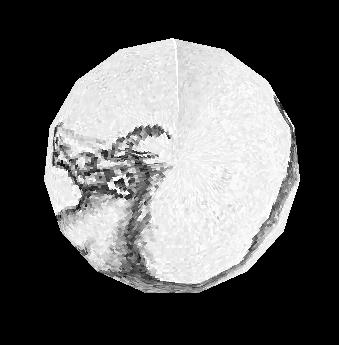
\includegraphics[width=0.7228in,height=0.7362in]{utr9/utr9-img014.jpg} 
 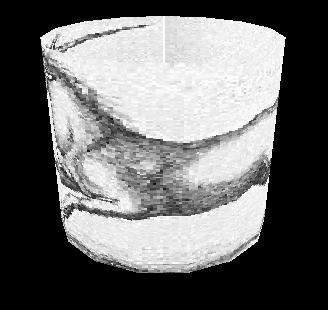
\includegraphics[width=0.7272in,height=0.6902in]{utr9/utr9-img015.jpg} \\\hline
{\selectlanguage{english} Filled Polygon}

~

~

~

~

{\selectlanguage{english} Line}

~

~

{\selectlanguage{english} Polygon}

~

~

~

{\selectlanguage{english} Segment} &
{\selectlanguage{english} The x and y texture coordinates are given by
p\textsubscript{1}x\textsubscript{0}+p\textsubscript{2}y\textsubscript{0}+p\textsubscript{3}z\textsubscript{0}+p\textsubscript{4}w\textsubscript{0}
} &
{\selectlanguage{english} A texture coordinate is assigned to a vertex. } &
 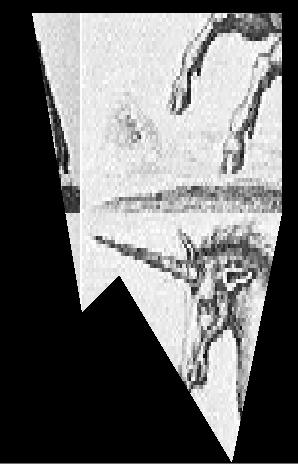
\includegraphics[width=0.6602in,height=0.7335in]{utr9/utr9-img016.jpg} 
 
\includegraphics[width=0.7228in,height=0.7516in]{utr9/utr9-img017.jpg} 
 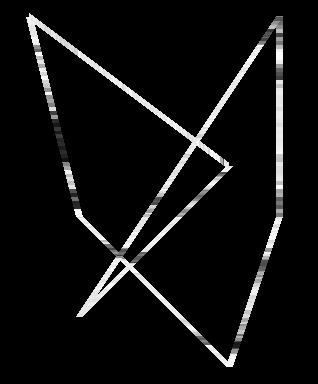
\includegraphics[width=0.7217in,height=0.8717in]{utr9/utr9-img018.jpg} 
 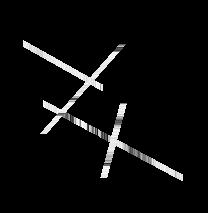
\includegraphics[width=0.7228in,height=0.7402in]{utr9/utr9-img019.jpg} \\\hline
{\selectlanguage{english} Torus} &
{\selectlanguage{english} The x and y texture coordinates are given by
p\textsubscript{1}x\textsubscript{0}+p\textsubscript{2}y\textsubscript{0}+p\textsubscript{3}z\textsubscript{0}+p\textsubscript{4}w\textsubscript{0}}
&
{\selectlanguage{english} None} &
 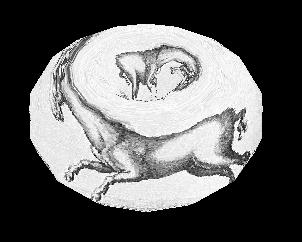
\includegraphics[width=0.8016in,height=0.6453in]{utr9/utr9-img020.jpg} \\\hline
\end{supertabular}
\end{center}


\subsection[2.8 Transparency and Blending]{2.8 Transparency and Blending}

Drawn 3D objects are normally fully opaque, obscuring anything drawn
behind them in a 3D scene. Transparency adjectives modify colors used
in material surfaces, allowing them to render objects that are not fully
opaque. The transparency adjectives are given in the following table,
progressing from solid to near-invisible.

\bigskip

{\centering\selectlanguage{english}\bfseries
Table 3 -- transparency adjectives
\par}

\begin{center}
\begin{tabular}{|l | l|}\hline
Transparency name & percent visible \\\hline
\texttt{opaque} & 100 \\
\texttt{dull}, a.k.a. \texttt{subtranslucent} & 75 \\
\texttt{translucent} & 50 \\
\texttt{subtransparent} & 25 \\
\texttt{transparent} & 5 \\\hline
\end{tabular}

\end{center}

\bigskip



When it is set \textsf{``on''}, the attribute \textsf{texmode} is used instead
of the current foreground color material specification; the two are
mutually exclusive by default.  Attribute \textsf{texmode} may instead be set
to \textsf{``texmode=blend''}, a mode in which the current color is
applied to the texture as it is output. By such a technique, a reddish
brick texture could for example be blended with green or blue to provide
bricks of different colors.


\section[3. Examples]{3. Examples}

The following section provides examples and a further description of
the Unicon 3D graphics facilities.

\subsection[3.1 Changing Context Attributes]{3.1 Changing Context Attributes}

As mentioned in the above design section, new context attributes have
been added to the Unicon 3D graphics facilities.  The user can change
these attributes throughout a program. To change from an attribute,
make a call to \textsf{WAttrib()} with the window to be drawn on, the
attributes to be changed, and their new values. Multiple attributes
can be changed with one call to \textsf{WAttrib()}. This is
illustrated in the following line of code, where the user changes the
eye position to \textsf{(0.0, 0.0, 5.0)} and the eye direction to look
at the positive z-axis on the window w. Since an assignment to
\textsf{eyepos}, \textsf{eyedir}, \textsf{eyeup} or \textsf{eye}
redraws the screen, it is important to note that the following will
redraw the scene once.


\bigskip

{\selectlanguage{english}\sffamily
WAttrib(w, ``eyepos=0.0,0.0,5.0'',``eyedir=0.0,0.0,1.0'')}


\bigskip

The values of the attributes can also be read by using the function
\textsf{WAttrib()}. By passing \textsf{WAttrib()} the window
and the name of the attribute to be read, the user will obtain the
value of the specified attributes. For example, to obtain the value of
the current eye position, call


\bigskip

{\selectlanguage{english}\sffamily
WAttrib(w, ``eyepos'')}


\bigskip

Multiple attributes can be read with one call to
\textsf{WAttrib()}. This is shown in the following line of code where
the user reads the current value of the eye direction and up direction.

\bigskip

{\selectlanguage{english}\sffamily
every put(attrList, WAttrib(w, ``eyedir'', ''eyeup'')}


\subsection[3.2 Drawing Primitives]{3.2 Drawing Primitives}

The following is an example on how to use some of the functions to
draw primitives.

\bigskip

{\selectlanguage{english}\sffamily
Fg(w, {\textquotedbl}ambient yellow{\textquotedbl})}

{\selectlanguage{english}\sffamily
\ \ \ \ \ \ DrawDisk(w, 0.4, -0.5, -4.0, 0.0, 1.0, 0.0, 0.0, 1.0, 0.5, -5.0, 0.5, 1.0) \ \ }

{\selectlanguage{english}\sffamily
\ \ \ \ \ Fg(w, {\textquotedbl}diffuse white{\textquotedbl})}

{\selectlanguage{english}\sffamily
\ \ \ \ \ DrawDisk(w, 0.4, -0.5, -4.0, 0.0, 1.0, 0.0, 225.0,1.0, 0.5, -5.0, 0.5,1.0,0.0,125.0)}

{\selectlanguage{english}\sffamily
\ \ \ \ \ \ Fg(w, {\textquotedbl}ambient pink{\textquotedbl})}

{\selectlanguage{english}\sffamily
\ \ \ \ \ \ DrawCylinder(w, \ 0.0, 1.0, -5.0, 1.0, 0.5, 0.3)}

{\selectlanguage{english}\sffamily
\ \ \ \ \ \ Fg(w, {\textquotedbl}specular navy{\textquotedbl})}

{\selectlanguage{english}\sffamily
\ \ \ \ \ \ DrawDisk(w, -0.5, -0.5, -2.0, 0.5, 0.3)}

{\selectlanguage{english}\sffamily
\ \ \ \ \ \ Fg(w, {\textquotedbl}emission green{\textquotedbl})}

{\selectlanguage{english}\sffamily
\ \ \ \ \ \ DrawSphere(w, 0.5, 1.0, -3.0, 0.5)}

{\selectlanguage{english}\sffamily
\ \ \ WAttrib(w, {\textquotedbl}light0=on, diffuse white{\textquotedbl})}

 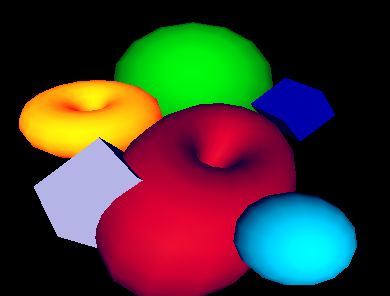
\includegraphics[width=2.8071in,height=2.1335in]{utr9/utr9-img021.png} 

The function \textsf{Fg()}, specifies the material properties of an
object. These material properties affect the color and appearance of
the primitives. After a call to \textsf{Fg()}, all objects will be
drawn with the material properties until the material property is
changed with another call to \textsf{Fg()}.\texttt{ }In this example,
a cube with a diffuse green material is drawn with sides of length
0.7. Then a sphere with a diffuse purple and ambient blue material is
drawn with radius 0.5 and center \textsf{(0.4, -0.5, -4.0)}. Next a
diffuse yellow and ambient grey torus with center
\textsf{(-1.0, 0.4, -4.0)}, an inner radius of 0.4, and an outer
radius of 0.5 is drawn. Finally a filled polygon with a diffuse red
material property and three vertices,\texttt{ }\textsf{(0.25, -0.25, -1.0)},
\textsf{(1.0, 0.25, -4.0)} and \textsf{(1.3, -0.4, -3.0)} is drawn.

\subsection[3.3 Slices and Rings]{3.3 Slices and Rings}

In many cases, it is useful to be able to control the level of detail
when drawing graphics primitives, for example depending on how far
away and/or how large the primitive is. Slices and rings attributes
serve this purpose. Both attributes take integer vales greater than 0
and denote how closely to approximate the abstract graphics shape when
rendering with simpler graphics primitives such as triangles or
quads. \textsf{WAttrib(``slices=10'', ``rings=10'')} for example sets
them both to 10. Greater values achieve smoother and more fine
detailed shapes but are more expensive to render, so these values
should be picked with care. These attributes can also be used to
achieve some useful effects, such as drawing a diamond using the the
\textsf{DrawSphere()} function or drawing a pyramid
using the \textsf{DrawCylinder()} function. \textsf{Slices} and
\textsf{rings} affect \textsf{DrawSphere()}, \textsf{DrawCylinder()},
\textsf{DrawTorus()} and \textsf{DrawDisk()} functions. The
example and figure below illustrates the use of
\textsf{slices} and \textsf{rings}.

{\selectlanguage{english}\sffamily
procedure main()}

{\selectlanguage{english}\sffamily
\ \ \ \&window := open({\textquotedbl}slices \& rings{\textquotedbl}, {\textquotedbl}gl{\textquotedbl},
{\textquotedbl}size=800,600{\textquotedbl}) {\textbar} stop({\textquotedbl}can't open window!{\textquotedbl})}


\bigskip

{\selectlanguage{english}\sffamily
\ \ \ Fg({\textquotedbl}blue{\textquotedbl}) \ }

{\selectlanguage{english}\sffamily
\ \ \ WAttrib( {\textquotedbl}slices=25{\textquotedbl}, {\textquotedbl}rings=25{\textquotedbl} ) \ \ }

{\selectlanguage{english}\sffamily
\ \ \ DrawSphere(-2.0, 2.0, 0, 0.5)}


\bigskip

{\selectlanguage{english}\sffamily
\ \ \ WAttrib( {\textquotedbl}slices=4{\textquotedbl}) \ \ }

{\selectlanguage{english}\sffamily
\ \ \ DrawSphere(-1.0, 2.0, 0, 0.5)}


\bigskip

{\selectlanguage{english}\sffamily
\ \ \ Rotate(45.0, 0, 1, 0)}

{\selectlanguage{english}\sffamily
\ \ \ DrawSphere( 0.0, 2.0, 0, 0.5)}

{\selectlanguage{english}\sffamily
\ \ \ Rotate(-45.0, 0, 1, 0)}


\bigskip

{\selectlanguage{english}\sffamily
\ \ \ WAttrib( {\textquotedbl}slices=25{\textquotedbl}, {\textquotedbl}rings=4{\textquotedbl}) \ \ }

{\selectlanguage{english}\sffamily
\ \ \ Fg({\textquotedbl}red{\textquotedbl}) \ }

{\selectlanguage{english}\sffamily
\ \ \ DrawSphere(-2.0, 0.5, 0, 0.5)}


\bigskip

{\selectlanguage{english}\sffamily
\ \ \ WAttrib( {\textquotedbl}slices=4{\textquotedbl}, {\textquotedbl}rings=4{\textquotedbl}) \ \ }

{\selectlanguage{english}\sffamily
\ \ \ DrawSphere(-1.0, 0.5, 0, 0.5)}


\bigskip

{\selectlanguage{english}\sffamily
\ \ \ Rotate(45.0, 0, 1, 0)}

{\selectlanguage{english}\sffamily
\ \ \ DrawSphere(0.0, 0.5, 0, 0.5)}

{\selectlanguage{english}\sffamily
\ \ \ Rotate(-45.0, 0, 1, 0)}


\bigskip

{\selectlanguage{english}\sffamily
\ \ \ WAttrib( {\textquotedbl}slices=25{\textquotedbl}, {\textquotedbl}rings=25{\textquotedbl}) \ \ }

{\selectlanguage{english}\sffamily
\ \ \ Fg({\textquotedbl}green{\textquotedbl}) \ }

{\selectlanguage{english}\sffamily
\ \ \ DrawCylinder(-2.0, -1, 0, .6, 0.5, 0.01)}


\bigskip

{\selectlanguage{english}\sffamily
\ \ \ WAttrib( {\textquotedbl}slices=4{\textquotedbl}, {\textquotedbl}rings=16{\textquotedbl}) \ \ }

{\selectlanguage{english}\sffamily
\ \ \ DrawCylinder(-1, -1, 0, .6, 0.5, 0.01)}


\bigskip

{\selectlanguage{english}\sffamily
\ \ \ Rotate(25.0, 0, 1, 0)}

{\selectlanguage{english}\sffamily
\ \ \ DrawCylinder(0, -1, 0, .6, 0.5, 0.01)}

{\selectlanguage{english}\sffamily
\ \ \ Rotate(-25.0, 0, 1, 0)}

{\selectlanguage{english}\sffamily
\ \ \ Eye( 0 , 0.5, 5.2, \ {}-1,0.66,0, \ 0,1,0 )}

{\selectlanguage{english}\sffamily
\ \ \ Refresh()}

{\selectlanguage{english}\sffamily
\ \ \ Event()}

{\selectlanguage{english}\sffamily
end}


\bigskip



\begin{center}
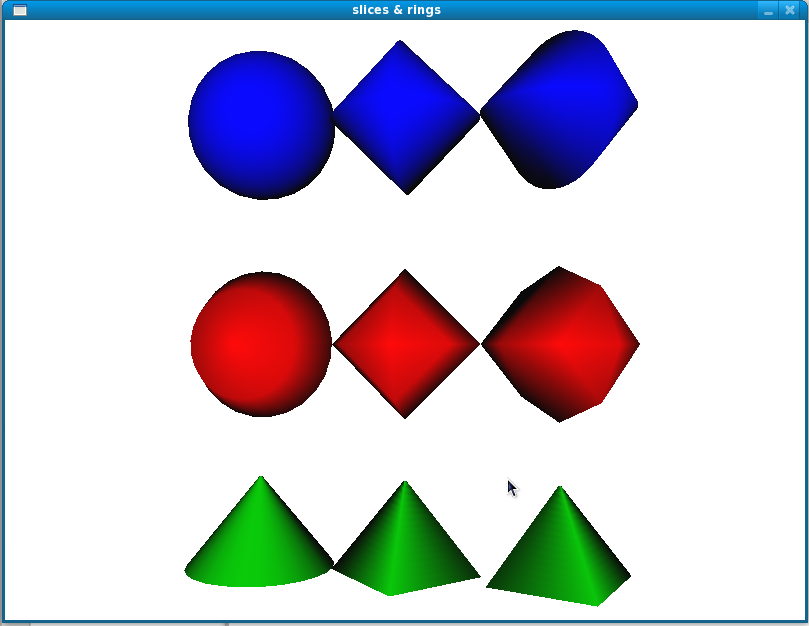
\includegraphics[width=3.148in,height=2.4299in]{utr9/utr9-img022.png}
\end{center}

\subsection[3.4 Lighting and Materials]{3.4 Lighting and Materials}


{\selectlanguage{english}
There are a maximum of eight lights that can be used in each scene of the Unicon 3D graphics facilities. The lights are
control by the context attributes \textsf{light0} through \textsf{light7}. Each light has five properties that can be
changed throughout the program, ambient, diffuse, specular, position, and on/off. The properties of a light can be
changed by using \textsf{WAttrib()} and one of \textsf{light0} through \textsf{light7}. To turn on or off a light,
one can assign \textsf{{}``on''} or \textsf{{}``off''} to the light, followed by a comma and a lighting value.
A lighting value is a string which contains one or more semi-colon separated lighting properties. A lighting property
is of the form

\bigskip

$\left[
\begin{array}{l}
diffuse\\ambient\\specular
\end{array}
\right]$ \textsf{\textit{color name}}

\bigskip

If one does not want to turn on or off a light, a lighting value is
specified. The following is a line of code which turns \textsf{light1}
on and gives it diffuse yellow and ambient gold lighting properties.

\bigskip

{\selectlanguage{english}
\ \ \textsf{WAttrib(w, ``light1=on, diffuse yellow; ambient gold'')}}

\bigskip

The following line of codes sets \textsf{light0} to the
default values for the lighting properties.

\bigskip

{\sffamily
WAttrib(w, ``light0=diffuse white; ambient black;}

{\selectlanguage{english}\sffamily
specular white; position 0.0, 1.0, 0.0'')}


\bigskip

The follow example shows the difference between the different types of
lighting that can be used in a scene. Each window is the same scene
rendered using different lighting. The upper right scene has an ambient
blue-green light. The upper left scene was drawn using a diffuse
blue-green light. The lower right scene uses only a specular blue-green
light. The scene in the lower left uses all three types of lighting.


\bigskip

{\centering  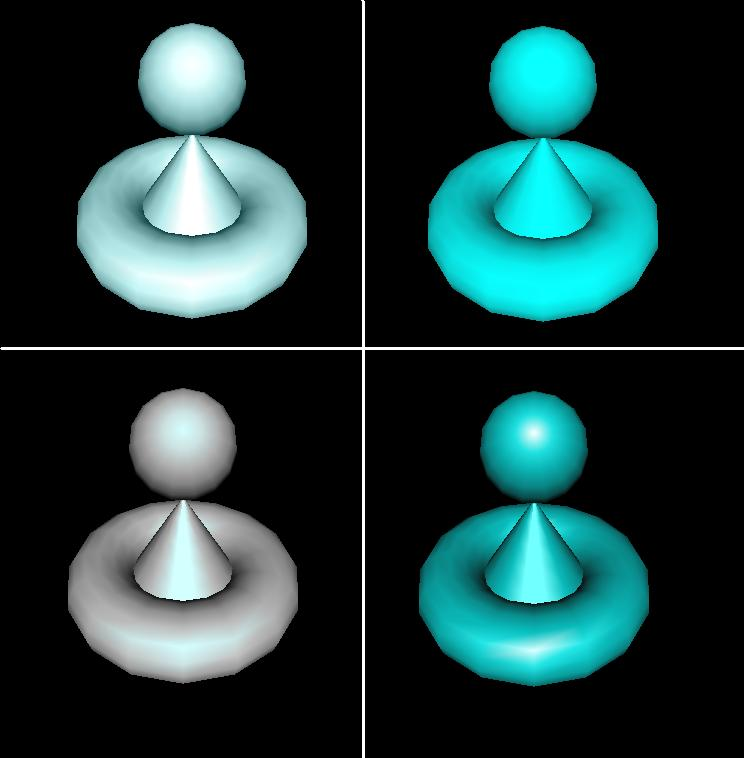
\includegraphics[width=2.1957in,height=2.2346in]{utr9/utr9-img023.jpg} \par}

\bigskip


\bigskip


\bigskip


\bigskip

{\selectlanguage{english}\sffamily
\ \ \ w := open({\textquotedbl}ambient.icn{\textquotedbl},{\textquotedbl}gl{\textquotedbl},
{\textquotedbl}bg=black{\textquotedbl}, {\textquotedbl}size=400,400{\textquotedbl})}

{\selectlanguage{english}\sffamily
\ \ \ WAttrib(w, {\textquotedbl}light0=on, ambient blue-green{\textquotedbl}, {\textquotedbl}fg=specular
white{\textquotedbl})}

{\selectlanguage{english}\sffamily
\ \ \ DrawCylinder(w, 0.0, -0.2, -3.5, 0.75, 0.5, 0.0)}

{\selectlanguage{english}\sffamily
\ \ \ DrawTorus(w,0.0, -0.2, -3.5, 0.3, 0.7)}

{\selectlanguage{english}\sffamily
\ \ \ DrawSphere(w,0.0, 0.59, -2.2, 0.3)}


\bigskip

{\selectlanguage{english}\sffamily
\ \ \ x := open({\textquotedbl}diffuse.icn{\textquotedbl},{\textquotedbl}gl{\textquotedbl},
{\textquotedbl}bg=black{\textquotedbl}, {\textquotedbl}size=400,400{\textquotedbl})}

{\selectlanguage{english}\sffamily
\ \ \ WAttrib(x, {\textquotedbl}light0=on, diffuse blue-green{\textquotedbl}, {\textquotedbl}fg=specular
white{\textquotedbl})}

{\selectlanguage{english}\sffamily
\ \ \ DrawCylinder(x, 0.0, -0.2, -3.5, 0.75, 0.5, 0.0)}

{\selectlanguage{english}\sffamily
\ \ \ DrawTorus(x,0.0, -0.2, -3.5, 0.3, 0.7)}

{\selectlanguage{english}\sffamily
\ \ \ DrawSphere(x, 0.0, 0.59, -2.2, 0.3)}


\bigskip

{\selectlanguage{english}\sffamily
\ \ \ y := open({\textquotedbl}specular.icn{\textquotedbl},{\textquotedbl}gl{\textquotedbl},
{\textquotedbl}bg=black{\textquotedbl}, {\textquotedbl}size=400,400{\textquotedbl})}

{\selectlanguage{english}\sffamily
\ \ \ WAttrib(y, {\textquotedbl}light0=on, specular blue-green{\textquotedbl}, {\textquotedbl}fg=specular
white{\textquotedbl})}

{\selectlanguage{english}\sffamily
\ \ \ DrawCylinder(y, 0.0, -0.2, -3.5, 0.75, 0.5, 0.0)}

{\selectlanguage{english}\sffamily
\ \ \ DrawTorus(y, 0.0, -0.2, -3.5, 0.3, 0.7)}

{\selectlanguage{english}\sffamily
\ \ \ DrawSphere(y, 0.0, 0.59, -2.2, 0.3)}


\bigskip

{\selectlanguage{english}\sffamily
\ \ \ z := open({\textquotedbl}all.icn{\textquotedbl},{\textquotedbl}gl{\textquotedbl},
{\textquotedbl}bg=black{\textquotedbl}, {\textquotedbl}size=400,400{\textquotedbl})}

{\selectlanguage{english}\sffamily
\ \ \ WAttrib(z, {\textquotedbl}light0=on, diffuse blue-green; specular blue-green; \_}

{\selectlanguage{english}\sffamily
\ \ \ \ \ \ \ \ \ \ \ \ \ \ \ \ \ \ \ \ \ \ \ \ \ \ \ \ \ \ \ \ \ \ \ \ \ \ \ \ \ ambient blue-green{\textquotedbl},
{\textquotedbl}fg=specular white{\textquotedbl})}

{\selectlanguage{english}\sffamily
\ \ \ DrawCylinder(z, 0.0, -0.2, -3.5, 0.75, 0.5, 0.0)}

{\selectlanguage{english}\sffamily
\ \ \ DrawTorus(z, 0.0, -0.2, -3.5, 0.3, 0.7)}

{\selectlanguage{english}\sffamily
\ \ \ DrawSphere(z, 0.0, 0.59, -2.2, 0.3)}


\bigskip

Materials can be changed using \textsf{Fg()} or \textsf{WAttrib()}
with the context attribute \textsf{fg}. A material value is a string
containing one or more semi-colon separated material
properties. Material properties are of the form

\bigskip

$\left[
\begin{array}{l}
diffuse\\ambient\\specular\\emission
\end{array}
\right]$ \textsf{\textit{color name}} or \textsf{``shininess n''},
where \textsf{n} is between \textsf{0} and \textsf{128}.

\bigskip

The default material property type is diffuse, so the call
\textsf{Fg({\textquotedbl}red{\textquotedbl})} is equivalent to
\textsf{Fg({\textquotedbl}diffuse red{\textquotedbl})}. For shininess,
a value of 0 spreads specular light broadly across an object and a
value of 128 focuses specular light at a single point. The following
line of code changes the current material property to diffuse green
and ambient orange.


\bigskip

{\selectlanguage{english}\ttfamily
\ \ \ \textsf{WAttrib(w, ``fg=diffuse green; ambient orange'')}}


\bigskip

{\selectlanguage{english}
The default values of the material properties are given in the following example. }


\bigskip

{\selectlanguage{english}\sffamily
Fg(w, ``diffuse light grey; ambient grey; \_}

{\selectlanguage{english}\sffamily
\ \ \ \ \ \ specular black; emission black; shininess 50'')}


\bigskip

The following is an example of several different material
properties used within one scene.

{\centering  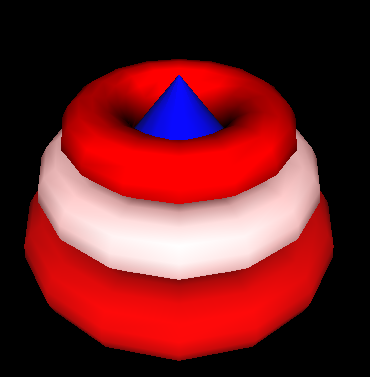
\includegraphics[width=1.6799in,height=1.7299in]{utr9/utr9-img024.png} \par}

\bigskip


\bigskip

{\selectlanguage{english}\sffamily
Fg(w, {\textquotedbl}diffuse blue{\textquotedbl})}

{\selectlanguage{english}\sffamily
DrawCylinder(w, 0.0, -0.2, -3.5, 1.2, 1.0, 0.0)}

{\selectlanguage{english}\sffamily
\ \ \ \ \ \ Fg(w, {\textquotedbl}diffuse red{\textquotedbl})}

{\selectlanguage{english}\sffamily
\ \ \ \ \ \ DrawTorus(w, 0.0, -0.2, -3.5, 0.3, 1.0)}

{\selectlanguage{english}\sffamily
\ \ \ \ \ \ Fg(w, {\textquotedbl}diffuse white; ambient red{\textquotedbl})}

{\selectlanguage{english}\sffamily
\ \ \ \ \ \ DrawTorus(w, 0.0, 0.2, -3.5, 0.3, 0.9)}

{\selectlanguage{english}\sffamily
\ \ \ \ \ \ Fg(w, {\textquotedbl}shininess 10; diffuse red; specular red; ambient black{\textquotedbl})}

{\selectlanguage{english}\sffamily
\ \ \ \ \ \ DrawTorus(w, 0.0, 0.55, -3.5, 0.3, 0.72)}


\bigskip

First a cylinder with a diffuse blue material is drawn. Then the
bottom torus is drawn, which has a diffuse red material. Next the
middle torus is draw with a diffuse white and ambient red
property. Finally the top torus is drawn with a diffuse red, specular
red and ambient property, and shininess of 10. Notice, that in order
an object not to be drawn with a previous material property, that
property must be reset to its default.

The following example shows the effects of emission color on an object.


\bigskip

{\centering  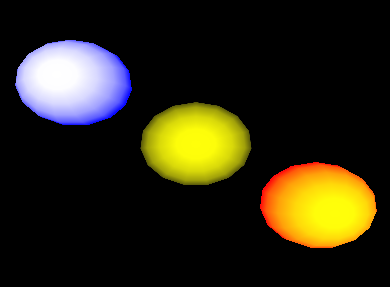
\includegraphics[width=2.4598in,height=1.8799in]{utr9/utr9-img025.png} \par}

\bigskip

{\selectlanguage{english}\sffamily
\ \ \ Fg(w, {\textquotedbl}emission blue; diffuse yellow{\textquotedbl}) }

{\selectlanguage{english}\sffamily
\ \ \ DrawSphere(w, -1.5, 1.0, -5.0, 0.7)}

{\selectlanguage{english}\sffamily
\ \ \ Fg(w, {\textquotedbl}emission black{\textquotedbl})}

{\selectlanguage{english}\sffamily
\ \ \ DrawSphere(w, 0.0, 0.0, -5.0, 0.7)}

{\selectlanguage{english}\sffamily
\ \ \ Fg(w, {\textquotedbl}emission red{\textquotedbl})}

{\selectlanguage{english}\sffamily
\ \ \ DrawSphere(w, 1.5, -1.0, -5.0, 0.7) }


\bigskip

In the above example, there are three diffuse yellow spheres drawn. If
an emission color of blue is applied to the sphere, the sphere appears
white with a blue ring. If the emission color is red, the sphere
remains yellow, but now has an orange-red ring. The middle sphere
shows the effect of having no emission color. Note that in order to
obtain the diffuse yellow sphere in the center, the emission color had
to be change to black. It was not needed to change the diffuse
material property.


\subsection[3.5 Textures]{3.5 Textures}

This section contains several examples of the use of textures in a
scene. There are several ways to specify the texture image in the
Unicon 3D graphics facilities: a file, an image string, or another
Unicon window. The following example shows how to use a file as a
texture. A .gif image of a map of the word is used to texture a
torus. The texture coordinates are the default coordinates as describe
in 2.7.


\bigskip

{\centering  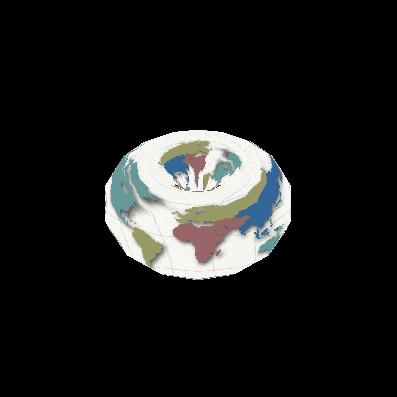
\includegraphics[width=2.0583in,height=2.0583in]{utr9/utr9-img026.jpg} \par}

\bigskip

{\selectlanguage{english}\ttfamily
\textsf{\ \ \ \ }\textsf{WAttrib(w, {\textquotedbl}texmode=on{\textquotedbl},
{\textquotedbl}texture=map.gif{\textquotedbl})}}

{\selectlanguage{english}\sffamily
\ \ \ \ DrawTorus(w, 0.0, 0.0, -3.0, 0.3, 0.4) }


\bigskip

{\selectlanguage{english}
Instead of using \textsf{WAttrib(w, {\textquotedbl}texture=map.gif{\textquotedbl})}\texttt{ }to specify the .gif file, a
call to \textsf{Texture(w, {\textquotedbl}map.gif{\textquotedbl})} could be used to obtain the same result.}


\bigskip

The next example illustrates the use of an image string to specify a
texture image. The format of the string is described in section
2.7. The string used for this example is taken from Graphics
Programming in Icon [Griswold98] page 156. This string is used as a
texture on a cube using the default texture coordinates.


\bigskip

{\centering  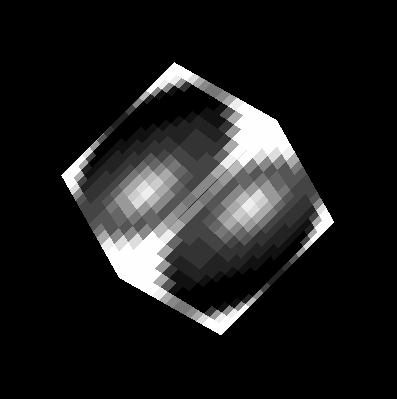
\includegraphics[width=2.0508in,height=2.0571in]{utr9/utr9-img027.jpg} \par}

\bigskip

{\selectlanguage{english}\sffamily
\ \ \ WAttrib(w, {\textquotedbl}texmode=on{\textquotedbl})}

{\selectlanguage{english}\sffamily
\ \ \ sphere:= {\textquotedbl}16,g16, FFFFB98788AEFFFF{\textquotedbl} {\textbar}{\textbar}}

{\selectlanguage{english}\sffamily
\ \ \ \ \ {\textquotedbl}FFD865554446AFFF FD856886544339FF E8579BA9643323AF{\textquotedbl}{\textbar}{\textbar}}

{\selectlanguage{english}\sffamily
\ \ \ \ \ {\textquotedbl}A569DECA7433215E 7569CDB86433211A 5579AA9643222108{\textquotedbl}{\textbar}{\textbar}}

{\selectlanguage{english}\sffamily
\ \ \ \ \ {\textquotedbl}4456776533221007 4444443332210007 4333333222100008{\textquotedbl}{\textbar}{\textbar}}

{\selectlanguage{english}\sffamily
\ \ \ \ \ {\textquotedbl}533322221100000A 822222111000003D D41111100000019F{\textquotedbl}{\textbar}{\textbar}}

{\selectlanguage{english}\sffamily
\ \ \ \ \ {\textquotedbl}FA200000000018EF FFA4000000028EFF FFFD9532248BFFFF{\textquotedbl}}

{\selectlanguage{english}\sffamily
\ \ \ Texture(w, sphere)}

{\selectlanguage{english}\sffamily
\ \ \ DrawCube(w, 0.0, 0.0, -3.0, 1.2)}


\bigskip

The next example shows the use of another Unicon window as a
texture. A simple scene of a lamp is drawn on the first window, which
is opened in \textsf{{}``gl''} mode. This window is then captured and
used as a texture on a cylinder. If a Unicon window opened in
\textsf{{}``g''}\texttt{ }mode as a texture the same method can be
used. Note that in the following code the first window is opened with
size 256 x 256. Texture images must have height and width that are
powers of 2, or the system must rescale them. The default coordinates
for cylinders are used.


\bigskip


\bigskip

{\centering\selectlanguage{english}
 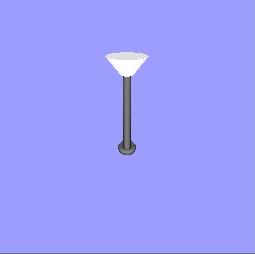
\includegraphics[width=1.4492in,height=1.4335in]{utr9/utr9-img028.jpg} \texttt{ \ \ }

\includegraphics[width=1.939in,height=1.952in]{utr9/utr9-img029.jpg} \texttt{ \ \ }
\par}


\bigskip


\bigskip

{\selectlanguage{english}\sffamily
w := open({\textquotedbl}win1{\textquotedbl},{\textquotedbl}gl{\textquotedbl},{\textquotedbl}bg=light
blue{\textquotedbl},{\textquotedbl}size=256,256{\textquotedbl})}

{\selectlanguage{english}\sffamily
\ \ \ \ \ Fg(w, {\textquotedbl}emission pale grey{\textquotedbl})}

{\selectlanguage{english}\sffamily
\ \ \ \ \ PushMatrix(w)}

{\selectlanguage{english}\sffamily
\ \ \ \ \ Rotate(w, -5.0, 1.0, 0.0, 0.0)}

{\selectlanguage{english}\sffamily
\ \ \ \ \ DrawCylinder(w, 0.0, 0.575, -2.0, 0.15, 0.05, 0.17)}

{\selectlanguage{english}\sffamily
\ \ \ \ \ PopMatrix(w) \ }

{\selectlanguage{english}\sffamily
\ \ \ \ \ Fg(w, {\textquotedbl}diffuse grey; emission black{\textquotedbl})}

{\selectlanguage{english}\sffamily
\ \ \ \ \ \ PushMatrix(w)}

{\selectlanguage{english}\sffamily
\ \ \ \ \ \ Rotate(w, -5.0, 1.0, 0.0, 0.0)}

{\selectlanguage{english}\sffamily
\ \ \ \ \ \ DrawCylinder(w, 0.0, 0.0, -2.5, 0.7, 0.035, 0.035)}

{\selectlanguage{english}\sffamily
\ \ \ \ \ \ PopMatrix(w) \ \ \ \ \ \ \ }

{\selectlanguage{english}\sffamily
\ \ \ \ \ \ DrawTorus(w, 0.0, -0.22, -2.5, 0.03, 0.06)}

{\selectlanguage{english}\sffamily
\ \ \ \ \ \ DrawTorus(w, 0.0, 0.6, -2.5, 0.05, 0.03)}


\bigskip

{\selectlanguage{english}\sffamily
w2 :=
open({\textquotedbl}win2.icn{\textquotedbl},{\textquotedbl}gl{\textquotedbl},{\textquotedbl}bg=black{\textquotedbl},{\textquotedbl}size=400,400{\textquotedbl})}

{\selectlanguage{english}\sffamily
\ \ \ \ WAttrib(w2, {\textquotedbl}texmode=on{\textquotedbl})}

{\selectlanguage{english}\sffamily
\ \ \ \ \ Texture(w2, w) }

{\selectlanguage{english}\sffamily
\ \ \ \ \ Fg(w2, {\textquotedbl}diffuse purple; ambient blue{\textquotedbl}) }

{\selectlanguage{english}\sffamily
DrawCylinder(w2, 0.0, 0.0, -3.5, 1.2, 0.7, \ 0.7)}


\bigskip

The next two examples illustrate the use of the default texture
coordinates versus texture coordinates specified by the programmer. In
both examples, a bi-level image is used as the texture image. The
format for such a string is described in section 2.7. This image is
taken from Graphics Programming in Icon [Griswold98] page 159. The
first example uses the default texture coordinates for a filled
polygon, which in this case is just a square with sides of length
one. In this case the default texture coordinates are as follows. The
coordinate \textsf{(0.0, 0.0) }of the texture image is mapped to the
vertex\texttt{ }\textsf{(0.0, 0.0, -2.0)} of the square, \textsf{(0.0,
  1.0) }is mapped to \textsf{(0.0, 1.0, -2.0), (1.0, 1.0)}\texttt{ }is
mapped to \textsf{(1.0, 1.0, -2.0)}, and \textsf{(1.0, 0.0) }is mapped
to \textsf{(1.0, 0.0, -2.0)}.


\bigskip

{\centering  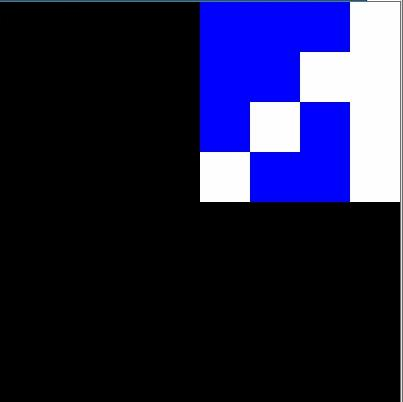
\includegraphics[width=1.8335in,height=1.8335in]{utr9/utr9-img030.jpg} \par}

\bigskip


\bigskip

{\selectlanguage{english}\sffamily
\ \ \ \ WAttrib(w, {\textquotedbl}fg=white{\textquotedbl}, {\textquotedbl}bg=blue{\textquotedbl},
{\textquotedbl}texmode=on{\textquotedbl}, {\textquotedbl}texture=4,\#8CA9{\textquotedbl})}

{\selectlanguage{english}\sffamily
\ \ \ \ Fg(w, {\textquotedbl}diffuse purple; ambient blue{\textquotedbl})}

{\selectlanguage{english}\sffamily
\ \ \ \ FillPolygon(w, 0.0, 0.0, -2.0, 0.0, 1.0, -2.0, 1.0, 1.0, -2.0, 1.0, 0.0, -2.0) }


\bigskip

This example uses the same texture image and the same object to be
textured, but instead uses the texture coordinates
\textsf{(0.0, 1.0)},\textsf{ (1.0, 1.0)},
\textsf{ (1.0, 1.0)}, and \textsf{(1.0, 0.0)}. So the
coordinate \textsf{(0.0, 1.0) }of the texture image is mapped to the
vertex \textsf{(0.0, 0.0, -2.0)} of the square, \textsf{(1.0, 1.0)}
is mapped to \textsf{(0.0, 1.0, -2.0),(1.0, 1.0)} is
mapped to \textsf{(1.0, 1.0, -2.0)}, and \textsf{(1.0}, \textsf{0.0)}
is mapped to \textsf{(1.0, 0.0, -2.0)}.


\bigskip

{\centering  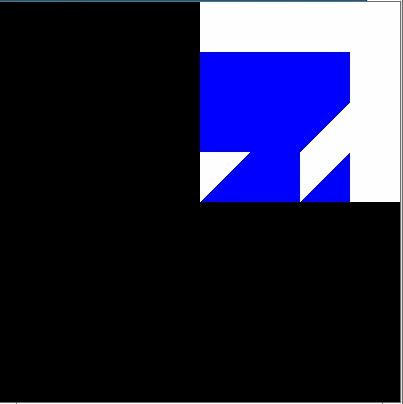
\includegraphics[width=2.0307in,height=2.0311in]{utr9/utr9-img031.jpg} \par}

\bigskip


\bigskip

{\selectlanguage{english}\sffamily
\ \ \ \ WAttrib(w, {\textquotedbl}fg=white{\textquotedbl}, {\textquotedbl}bg=blue{\textquotedbl},
{\textquotedbl}texmode=on{\textquotedbl},}

{\selectlanguage{english}\sffamily
\ \ \ \ \ \ \ \ \ \ \ \ \ \ \ \ \ {\textquotedbl}texcoord=0.0, 1.0, 1.0, 1.0, 1.0, 1.0, 1.0, 0.0{\textquotedbl},
{\textquotedbl}texture=4,\#8CA9{\textquotedbl})}

{\selectlanguage{english}\sffamily
\ \ \ \ FillPolygon(w, 0.0, 0.0, -2.0, 0.0, 1.0, -2.0, 1.0, 1.0, -2.0, 1.0, 0.0, -2.0) }


\bigskip

Also instead of using \textsf{WAttrib()} with the attribute
\textsf{texcoord}, the function \textsf{Texcoord()} could be
used. So the line

\bigskip

{\selectlanguage{english}\sffamily
WAttrib(w,{\textquotedbl}texcoord=0.0, 1.0, 1.0, 1.0, 1.0, 1.0,1.0, 0.0{\textquotedbl})}


\bigskip

\noindent could be replaced by


\bigskip

{\selectlanguage{english}\sffamily
Texcoord(w, 0.0, 1.0, 1.0, 1.0, 1.0, 1.0,1.0, 0.0)\newline
}

\subsection[3.6 A Larger Textures Example]{3.6 A Larger Textures Example}

The following is a more complicated example that uses many features of
the Unicon 3D graphics facilities described in the previous
sections. This example also illustrates the effect that adding texture
to a scene can have. The scene on the left is a scene drawn without
any texturing. The scene on the right contains texturing. The scene on
the right is a much more realistic scene than the one on the left.

All textures used in the textured scene, except for the unicorn, where
captured using a digital camera. These images were then converted into
.gif files and scaled to width and height of 2\textsuperscript{n}.
Directly using an image file is one feature of the Unicon 3D graphics
facilities that makes adding textures simpler than using OpenGL.


\bigskip

{\selectlanguage{english}
 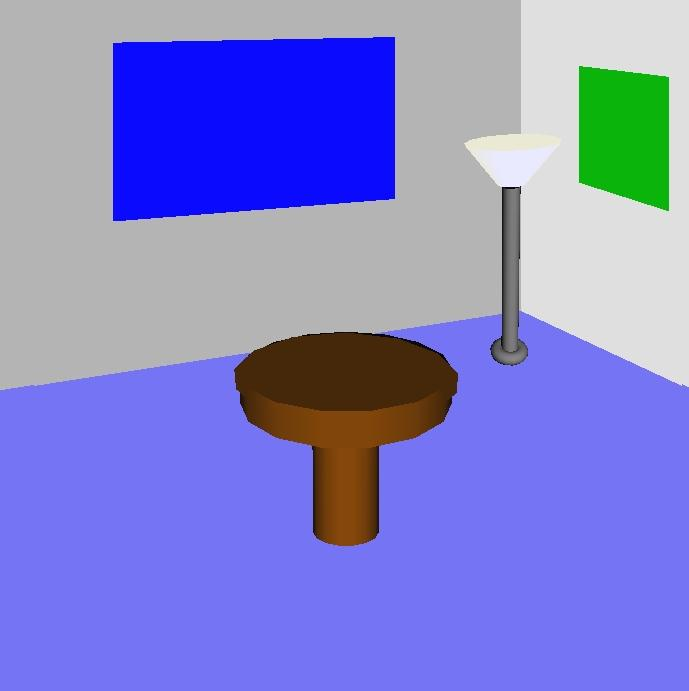
\includegraphics[width=2.6543in,height=2.6693in]{utr9/utr9-img032.jpg} \textbf{ \ \ \ \ \ \ \ \ \ \ \ \ \ }
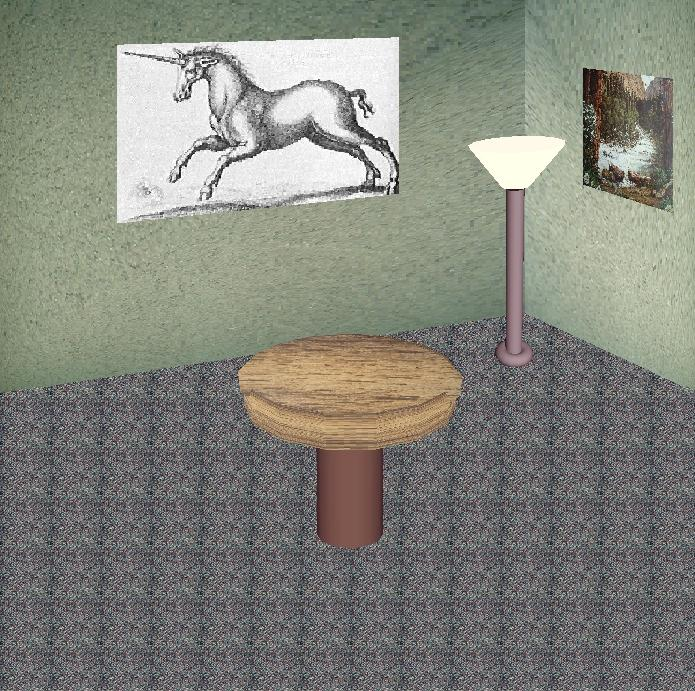
\includegraphics[width=2.6846in,height=2.6693in]{utr9/utr9-img033.jpg} }

\ \ \ \ \ \ \ \ \ \ \ \ \ \ \ \ \ 
An untextured scene \hfill A textured scene
\ \ \ \ \ \ \ \ \ \ \ \ \ \ \ \ \ 


\bigskip

{\selectlanguage{english}\sffamily
procedure main()}

{\selectlanguage{english}\sffamily
\ \ \ \&window
:=open({\textquotedbl}textured.icn{\textquotedbl},{\textquotedbl}gl{\textquotedbl},{\textquotedbl}bg=black{\textquotedbl},{\textquotedbl}size=700,700{\textquotedbl})}


\bigskip

{\selectlanguage{english}\sffamily
\ \ \ \# Draw the floor of the room}

{\selectlanguage{english}\sffamily
\ \ \ WAttrib({\textquotedbl}texmode=on{\textquotedbl}, {\textquotedbl}texture=carpet.gif{\textquotedbl})}

{\selectlanguage{english}\sffamily
\ \ \ FillPolygon(-7.0, -0.9, -14.0, -7.0, -7.0, -14.0,}

{\selectlanguage{english}\sffamily
\ \ \ \ \ \ \ \ \ \ \ \ \ \ \ \ \ \ \ \ \ \ \ 7.0, -7.0, -14.0, 7.0, -0.9, -14.0, 3.5, 0.8, -14.0)}


\bigskip

{\selectlanguage{english}\sffamily
\ \ \ \# Draw the right wall}

{\selectlanguage{english}\sffamily
\ \ \ WAttrib({\textquotedbl}texture=wall1.gif{\textquotedbl}, {\textquotedbl}texcoord=0.0, 1.0, 0.0, 0.0, 1.0, 0.0,
1.0, 1.0{\textquotedbl})}

{\selectlanguage{english}\sffamily
\ \ \ FillPolygon(2.0, 4.0, -8.0, 8.3, 8.0, -16.0, 8.3, -1.2, -16.0, 2.0, 0.4, -8.0)}


\bigskip

{\selectlanguage{english}\sffamily
\ \ \ \# Draw the left wall}

{\selectlanguage{english}\sffamily
\ \ \ WAttrib({\textquotedbl}texture=wall2.gif{\textquotedbl})}

{\selectlanguage{english}\sffamily
\ \ \ FillPolygon(2.0, 4.0 ,-8.0, -9.0, 8.0, -16.0, -9.0,-1.2,-16.0, 2.0, 0.4, -8.0)}


\bigskip

{\selectlanguage{english}\sffamily
\ \ \ \# Draw a picture}

{\selectlanguage{english}\sffamily
\ \ \ WAttrib({\textquotedbl}texture=poster.gif{\textquotedbl}, {\textquotedbl}texcoord=0.0, 1.0, 0.0, 0.0, 1.0, 0.0,
1.0, 1.0{\textquotedbl})}

{\selectlanguage{english}\sffamily
\ \ \ FillPolygon(1.0, 1.2, -3.0, 1.0, 0.7, -3.0, 1.2, 0.5, -2.6, 1.2, 1.0, -2.6)}


\bigskip

{\selectlanguage{english}\sffamily
\ \ \ \# Draw another picture}

{\selectlanguage{english}\sffamily
\ \ \ WAttrib({\textquotedbl}texture=unicorn.gif{\textquotedbl}, {\textquotedbl}texcoord=1.0, 0.0, 0.0, 0.0, 0.0, 1.0,
1.0, 1.0{\textquotedbl})}

{\selectlanguage{english}\sffamily
\ \ \ FillPolygon(0.8, 2.0, -9.0, -3.0, 1.6, -9.0, 3.0, 3.9,-9.0, 0.8, 4.0, -9.0)}


\bigskip

{\selectlanguage{english}\sffamily
\ \ \ \# Draw the lamp}

{\selectlanguage{english}\sffamily
\ \ \ WAttrib({\textquotedbl}texmode=off{\textquotedbl})}

{\selectlanguage{english}\sffamily
\ \ \ PushMatrix()}

{\selectlanguage{english}\sffamily
\ \ \ Translate(0.7, 0.20, -0.5)}

{\selectlanguage{english}\sffamily
\ \ \ Fg({\textquotedbl}emission pale weak yellow{\textquotedbl})}

{\selectlanguage{english}\sffamily
\ \ \ PushMatrix()}

{\selectlanguage{english}\sffamily
\ \ \ Rotate(-5.0, 1.0, 0.0, 0.0)}

{\selectlanguage{english}\sffamily
\ \ \ Rotate( 5.0, 0.0, 0.0, 1.0)}

{\selectlanguage{english}\sffamily
\ \ \ DrawCylinder(-0.05, 0.570, -2.0, 0.15, 0.05, 0.17)}

{\selectlanguage{english}\sffamily
\ \ \ PopMatrix()}

{\selectlanguage{english}\sffamily
\ \ \ Fg({\textquotedbl}diffuse grey; emission black{\textquotedbl})}

{\selectlanguage{english}\sffamily
\ \ \ PushMatrix()}

{\selectlanguage{english}\sffamily
\ \ \ Rotate(-5.0, 1.0, 0.0, 0.0)}

{\selectlanguage{english}\sffamily
\ \ \ Rotate( 6.0, 0.0, 0.0, 1.0)}

{\selectlanguage{english}\sffamily
\ \ \ DrawCylinder(0.0, 0.0, -2.5, 0.7, 0.035, 0.035)}

{\selectlanguage{english}\sffamily
\ \ \ PopMatrix()}

{\selectlanguage{english}\sffamily
\ \ \ PushMatrix()}

{\selectlanguage{english}\sffamily
\ \ \ Rotate(6.0, 0.0, 0.0, 1.0)}

{\selectlanguage{english}\sffamily
\ \ \ DrawTorus(-0.02, -0.22, -2.5, 0.03, 0.05)}

{\selectlanguage{english}\sffamily
\ \ \ PopMatrix() }

{\selectlanguage{english}\sffamily
\ \ \ PopMatrix()}


\bigskip

{\selectlanguage{english}\sffamily
\ \ \ \# Draw the table }

{\selectlanguage{english}\sffamily
\ \ \ WAttrib({\textquotedbl}texcoord=auto{\textquotedbl}, {\textquotedbl}texmode=on{\textquotedbl},
{\textquotedbl}texture=table.gif{\textquotedbl})}


\bigskip

{\selectlanguage{english}\sffamily
\ \ \ PushMatrix()}

{\selectlanguage{english}\sffamily
\ \ \ Rotate(-10.0, 1.0, 0.0,0.0)}

{\selectlanguage{english}\sffamily
\ \ \ DrawCylinder(0.0, 0.2, -2.0, 0.1, 0.3, 0.3)}

{\selectlanguage{english}\sffamily
\ \ \ PopMatrix()}


\bigskip

{\selectlanguage{english}\sffamily
\ \ \ PushMatrix()}

{\selectlanguage{english}\sffamily
\ \ \ Translate(0.0, -0.09, -1.8)}

{\selectlanguage{english}\sffamily
\ \ \ Rotate(65.0, 1.0, 0.0, 0.0)}

{\selectlanguage{english}\sffamily
\ \ \ DrawDisk(0.0, 0.0, 0.0, 0.0, 0.29) }

{\selectlanguage{english}\sffamily
\ \ \ PopMatrix()}


\bigskip

{\selectlanguage{english}\sffamily
\ \ \ WAttrib({\textquotedbl}texmode=off{\textquotedbl}, {\textquotedbl}fg=diffuse weak brown{\textquotedbl})}

{\selectlanguage{english}\sffamily
\ \ \ PushMatrix()}

{\selectlanguage{english}\sffamily
\ \ \ Rotate(-20.0, 1.0, 0.0,0.0)}

{\selectlanguage{english}\sffamily
\ \ \ DrawCylinder(0.0, 0.2, -2.2, 0.3, 0.1, 0.1)}

{\selectlanguage{english}\sffamily
\ \ \ PopMatrix()}

{\selectlanguage{english}\sffamily
\ \ \ while (e := Event()) \~{}== {\textquotedbl}q{\textquotedbl} do \{}

{\selectlanguage{english}\sffamily
\ \ \ \ \ \ write(image(e), {\textquotedbl}: {\textquotedbl}, \&x, {\textquotedbl},{\textquotedbl}, \&y)}

{\selectlanguage{english}\sffamily
\ \ \ \ \ \ \}}

{\selectlanguage{english}\sffamily
end}


\bigskip

In order to apply textures to the scene, texturing must first be
turned on. Next, the texture to be applied is specified. Then the
floor of the scene is drawn, which is done by using a filled
polygon. The default texture coordinates are used to apply the carpet
texture to the floor of the room. The tiled appearance on the floor of
the room is caused by the use of the default texture coordinates. This
can be avoided by using user defined texture coordinates. This is what
is done for the textures that are applied to the two walls of the room
and the pictures.

The lamp does not have any texturing applied to it, so it is necessary
to turn off texturing before drawing the lamp.  Also for the lamp to
be centered properly in the room, transformations are used. Notice the
use of matrices to isolate the transformations of the lamp. Finally to
draw the table with a textured top and an untextured base, two
cylinders and a disk are used. Texturing is applied to a cylinder and
the disk. Notice the call

{\selectlanguage{english}
\ \ \ \textsf{WAttrib(w, {\textquotedbl}texcoord=auto{\textquotedbl})}}

This resets the texture coordinates to the defaults. Finally,
texturing is turned off to draw the base of the table.


\subsection[3.7 Animation]{3.7 Animation}

Graphics animation is performance sensitive, and Unicon is
substantially slower than lower level systems programming languages
such as C and C++. Nevertheless, it is possible to prototype simple 3D
animations using Unicon; applications with few moving objects can
achieve smooth animation with acceptable frame rates.

In OpenGL, animations are normally written to redraw the entire scene
each time any object has moved, or the user has changed point of
view. An application can repeatedly call \textsf{EraseArea()}
followed by the
appropriate graphics primitives to achieve this effect, but the
results often appear to flicker. It is better to let OpenGL's built-in
double buffering, and Unicon's runtime system, do the
redrawing. Unicon maintains a \textit{display list} of graphics
operations to execute whenever the screen must be redrawn; these
operations are effectively everything since the last EraseArea(). The
display list for a window can be obtained by calling
WindowContents(). The elements of the list are Unicon records and
lists containing the string names and parameters of graphics
primitives. For example, a call to \textsf{DrawSphere(w,x,y,z,r)}
returns (and adds to the display list) a record
gl\_sphere(``DrawSphere'', x, y, z, r). Instead of redrawing the
entire scene in order to move an object,
you can modify its display list record and call \textsf{Refresh()}.  The
following code fragment illustrates animation by causing a ball to
slide up and down. In order to ``bounce'' the program would need to
incorporate physics.

\bigskip

{\selectlanguage{english}\sffamily
sphere := DrawSphere(w, x, y, z, r)}

{\selectlanguage{english}\sffamily
increment := 0.2}

{\selectlanguage{english}\sffamily
every i := 1 to 100 do \{}

{\selectlanguage{english}\sffamily
\ \ \ every j := 1 to 100 do \{}

{\selectlanguage{english}\sffamily
\ \ \ \ \ \ sphere.y +:= increment}

{\selectlanguage{english}\sffamily
\ \ \ \ \ \ Refresh(w)}

{\selectlanguage{english}\sffamily
\ \ \ \ \ \ \}}

{\selectlanguage{english}\sffamily
\ \ \ \}}

\bigskip

\noindent
This technique gives animation rates of 100-200 frames per second in
simple tests on current midrange PC hardware, indicating that the
system will support smooth animation, at least for small numbers of
objects.


\subsection[3.8 Object Selection]{3.8 Object Selection}

Many 3D applications allow the user to interact with, select, or
identify 3D objects in a scene by clicking on objects with the
mouse. In Unicon, a window attribute (\texttt{pick}) enables or
disables 3D selection. When pick=on, keyword \texttt{\&pick} can be
used to access the 3D selection results. The function (WSection()) is
used to name objects in the scene. The steps required to use 3D
selection in Unicon are summarized by the following:

\bigskip

\begin{itemize}
\item Enable the selection
\item Give selectable 3D objects unique string names
\item Collect selection results through the keyword \textsf{\&pick}
\end{itemize}

\bigskip

Although this section uses the word ``selection'' freely to refer to
3D object selection, the Unicon language consistently uses ``pick''
instead of ``select'' for 3D objects. The reason for this is that
``selection'' is used in other ways in computing systems and user
interfaces. In Unicon and in certain window systems, it refers to the
mechanism used when data is copied and pasted between applications.


\subsubsection[3.8.1 Controlling the selection state]{3.8.1 Controlling the selection state}

Attribute \textsf{{}``pick''} turns on or off selection within
portions of a rendered scene. To turn on 3D selection at any point in
the program, the following statement should be inserted at that
point:


\bigskip

{\selectlanguage{english}\sffamily
WAttrib({\textquotedbl}pick=on{\textquotedbl})}


\bigskip

{\selectlanguage{english}
To turn off the 3D selection, simply make another call to \textsf{WAttrib()}:}


\bigskip

{\selectlanguage{english}\sffamily
WAttrib({\textquotedbl}pick=off{\textquotedbl})}


\bigskip

To check the current 3D selection state (on or off), the function
\texttt{WAttrib} can be called with the string parameter
\textsf{{\textquotedbl}pick{\textquotedbl}} (i.e
\textsf{WAttrib(``pick'')} ) and it will return a string value of
\textsf{{\textquotedbl}on{\textquotedbl}} or
\textsf{{\textquotedbl}off{\textquotedbl}} depending on the current 3D
selection state. By default 3D selection is turned off. The program
can turn on and off the 3D selection depending on the program
requirements. For a better performance, selection should be turned off
for all non-selectable objects in the scene.


\subsubsection[3.8.2 Naming 3D objects]{3.8.2 Naming 3D objects}

3D Objects are defined by their corresponding rendered primitives. The
function \textsf{WSection()} marks the beginning and the ending of a
section that holds a 3D object. A call to \textsf{WSection()} with a
parameter string marks the beginning of a 3D object with the string as
its name. Another call to \textsf{WSection} with no string parameter
marks the end of the 3D objects. All of the rendered graphics between
a beginning \textsf{WSection()} and its corresponding ending
\textsf{WSection} are parts of the same object. To make it selectable,
a 3D object must have at least one graphical primitive. A line or a
sphere are examples of such primitives. The string name should be
unique to distinguish different objects from each other. Different
objects could have the same name if the same action would be taken no
matter which of these objects is picked. The following code fragment
is an example of named 3D objects. It simply draws a red rectangle and
gives it the name {\textquotedbl}redrect{\textquotedbl}.


\bigskip

{\selectlanguage{english}\sffamily
WSection({\textquotedbl}redrect{\textquotedbl})\ \ \# beginning of a new object named redrect}

{\selectlanguage{english}\sffamily
Fg({\textquotedbl}red{\textquotedbl}) \ }

{\selectlanguage{english}\sffamily
FillPolygon(0,0,0, 0,1,0, 1,1,0, 1,0,0)}

{\selectlanguage{english}\sffamily
WSection()\ \ \ \ \ \ \# end of the object redrect}


\bigskip

In the example above
\textsf{WSection({\textquotedbl}redrect{\textquotedbl})} marks the
beginning of a new object with the name
redrect. \textsf{Fg({\textquotedbl}red{\textquotedbl})} doesn't affect
selection because it doesn't produce a rendered
object. \textsf{FillPolygon(0,0,0, 0,1,0, 1,1,0, 1,0,0)} on the other
hand does affect selection because it produces a rendered object, and
it actually represents the object named redrect.
\textsf{WSection()} marks the end of the object named redrect.


\subsubsection[3.8.3 Retrieving picked objects]{3.8.3 Retrieving picked objects}

The keyword \textsf{\&pick} generates the names of objects that were
clicked on at the last returned event, if they were associated with a
name using \textsf{WSection(name)}. A given mouse click might
correspond to multiple objects that are rendered along the ray from
the camera through the point clicked. In addition, \textsf{WSection()}
calls may be nested, in which case the name reported by
\textsf{\&pick} will be a concatenation (separated by hyphens) of the
\textsf{WSection()} names enclosing the object clicked. The following
code fragment writes all of the objects names that were picked by the
mouse click:


\bigskip

{\selectlanguage{english}\sffamily
every picked\_object := \&pick do}

{\selectlanguage{english}\sffamily
\ \ \ write({\textquotedbl} picked object :{\textquotedbl}, picked\_object)}


\bigskip

If there were no selectable objects under the cursor at the time of
the event, \textsf{\&pick} just fails and produces no
results. \textsf{\&pick} gets its results from both left-clicks and
right-clicks.

\bigskip

These ideas are illustrated in the following example, which draws
a crude humanoid figure. The rendering function turns
\textsf{{}``pick=on''} and then uses \textsf{WSection()} calls to
identify different parts of the figure.


\begin{center}
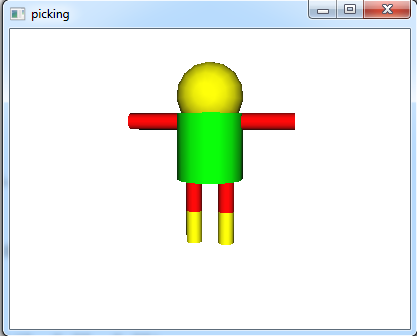
\includegraphics[width=2.3402in,height=1.8799in]{utr9/utr9-img034.png}
\end{center}

\bigskip


\bigskip

{\selectlanguage{english}\sffamily
procedure drawman()}

{\selectlanguage{english}\sffamily
\ \ \ h := 2.0}

{\selectlanguage{english}\sffamily
\ \ \ WAttrib({\textquotedbl}pick=on{\textquotedbl})}

{\selectlanguage{english}\sffamily
\ \ \ WSection({\textquotedbl}man{\textquotedbl})}

{\selectlanguage{english}\sffamily
\ \ \ \ \ \ WSection({\textquotedbl}body{\textquotedbl})}

{\selectlanguage{english}\sffamily
\ \ \ \ \  Fg({\textquotedbl}green{\textquotedbl})}

{\selectlanguage{english}\sffamily
\ \ \ \ \  DrawCylinder(0, 0, 0, h, 1.0, 1.0)}

{\selectlanguage{english}\sffamily
\ \ \ \ \ \ WSection()}

{\selectlanguage{english}\sffamily
\ \ \ \ \ \ WSection({\textquotedbl}head{\textquotedbl})}

{\selectlanguage{english}\sffamily
\ \ \ \ \  Fg({\textquotedbl}yellow{\textquotedbl})}

{\selectlanguage{english}\sffamily
\ \ \ \ \  DrawSphere(0.0,h+0.5,0.0, 1.0)}

{\selectlanguage{english}\sffamily
\ \ \ \ \ \ WSection()}

{\selectlanguage{english}\sffamily
\ \ \ \ \ \ WSection({\textquotedbl}rightleg{\textquotedbl})}

{\selectlanguage{english}\sffamily
\ \ \ \ \ \ WSection({\textquotedbl}upperrightleg{\textquotedbl})}

{\selectlanguage{english}\sffamily
\ \  Fg({\textquotedbl}red{\textquotedbl})}

{\selectlanguage{english}\sffamily
\ \  DrawCylinder(-0.5, -h/2, 0, h/2, 0.25, 0.25)}

{\selectlanguage{english}\sffamily
\ \ \ \ \ \ WSection()}

{\selectlanguage{english}\sffamily
\ \ \ \ \ \ WSection({\textquotedbl}lowerrightleg{\textquotedbl})}

{\selectlanguage{english}\sffamily
\ \  Fg({\textquotedbl}yellow{\textquotedbl})}

{\selectlanguage{english}\sffamily
\ \  DrawCylinder(-0.5, -h, 0, h/2, 0.25, 0.25)}

{\selectlanguage{english}\sffamily
\ \ \ \ \ \ WSection()}

{\selectlanguage{english}\sffamily
\ \ \ \ \ \ WSection()}

{\selectlanguage{english}\sffamily
\ \ \ \ \ \ WSection({\textquotedbl}leftleg{\textquotedbl})}

{\selectlanguage{english}\sffamily
\ \  WSection({\textquotedbl}upperleftleg{\textquotedbl})\ \ }

{\selectlanguage{english}\sffamily
\ \  \ \ \ Fg({\textquotedbl}red{\textquotedbl})}

{\selectlanguage{english}\sffamily
\ \ \ \ \  \ \ \ DrawCylinder(0.5, -h/2, 0, h/2, 0.25, 0.25)}

{\selectlanguage{english}\sffamily
\ \ \ \ \  WSection()}

{\selectlanguage{english}\sffamily
\ \  WSection({\textquotedbl}lowerleftleg{\textquotedbl})\ }

{\selectlanguage{english}\sffamily
\ \  \ \ \ Fg({\textquotedbl}yellow{\textquotedbl})}

{\selectlanguage{english}\sffamily
\ \ \ \ \  \ \ \ DrawCylinder(0.5, -h, 0, h/2, 0.25, 0.25)}

{\selectlanguage{english}\sffamily
\ \ \ \ \  WSection()}

{\selectlanguage{english}\sffamily
\ \ \ \ \ \ WSection()}

{\selectlanguage{english}\sffamily
\ \ \ \ \ \ PushMatrix()}

{\selectlanguage{english}\sffamily
\ \ \ \ \  Translate(0.5, h-0.25, 0.0)}

{\selectlanguage{english}\sffamily
\ \ \ \ \  Rotate(-90, 0, 0, 1)}

{\selectlanguage{english}\sffamily
\ \ \ \ \  WSection({\textquotedbl}leftarm{\textquotedbl})}

{\selectlanguage{english}\sffamily
\ \ \ \ \  \ \ \ Fg({\textquotedbl}red{\textquotedbl})}

{\selectlanguage{english}\sffamily
\ \ \ \ \  \ \ \ DrawCylinder(0, 0, 0, h, 0.25, 0.25)}

{\selectlanguage{english}\sffamily
\ \ \ \ \  WSection()}

{\selectlanguage{english}\sffamily
\ \ \ \ \ \ PopMatrix()}

{\selectlanguage{english}\sffamily
\ \ \ \ \ PushMatrix()}

{\selectlanguage{english}\sffamily
\ \ \ \ \ Translate(-0.5, h-0.25, 0.0)}

{\selectlanguage{english}\sffamily
\ \ \ \ \ Rotate(90, 0, 0, 1)}

{\selectlanguage{english}\sffamily
\ \ \ \ \ WSection({\textquotedbl}rightarm{\textquotedbl})}

{\selectlanguage{english}\sffamily
\ \ \ \ \  \ \ Fg({\textquotedbl}red{\textquotedbl})}

{\selectlanguage{english}\sffamily
\ \ \ \ \  \ \ DrawCylinder(0, 0, 0, h, 0.25, 0.25)}

{\selectlanguage{english}\sffamily
\ \ \ \ \ WSection()}

{\selectlanguage{english}\sffamily
\ \ \ \ \ PopMatrix()}

{\selectlanguage{english}\sffamily
\ \ \ WSection()}

{\selectlanguage{english}\sffamily
end}


\bigskip

The event-handling code for \textsf{\&lpress} looks in \textsf{\&pick}
to see what (if anything) the user was selecting.

\bigskip

{\selectlanguage{english}\sffamily
procedure main()}

{\selectlanguage{english}\sffamily
\ \ \ \&window := w := open({\textquotedbl}picking{\textquotedbl} , {\textquotedbl}gl{\textquotedbl},
{\textquotedbl}size=400,300{\textquotedbl}) {\textbar}}

{\selectlanguage{english}\sffamily
\ \ \ \ \ \ stop({\textquotedbl} failed to open 3d window! {\textquotedbl})}

{\selectlanguage{english}\sffamily
\ \ \ drawman()}

{\selectlanguage{english}\sffamily
\ \ \ Eye(-2,1.8,-12, \ 0,0,0, \ 0,1,0 )}

{\selectlanguage{english}\sffamily
\ \ \ Refresh(w)}

{\selectlanguage{english}\sffamily
\ \ \ repeat \{}

{\selectlanguage{english}\sffamily
\ \ \ \ \ \ case e := Event(w) of\{}

{\selectlanguage{english}\sffamily
\ \  {\textquotedbl}q{\textquotedbl}{\textbar}{\textquotedbl}{\textbackslash}e{\textquotedbl} : \{ return \}
\ \ \ \ \ \ \ \ \ }

{\selectlanguage{english}\sffamily
\ \  \&lpress : \{\  \ }

{\selectlanguage{english}\sffamily
\ \  \ \ \ write({\textquotedbl} mouse click{\textquotedbl} )}

{\selectlanguage{english}\sffamily
\ \  \ \ \ every item := \&pick do\{}

{\selectlanguage{english}\sffamily
\ \  \ \ \ \ \ \ write( {\textquotedbl}on part:{\textquotedbl}, item)}

{\selectlanguage{english}\sffamily
\ \  \ \ \ \}}

{\selectlanguage{english}\sffamily
\ \  \}}

{\selectlanguage{english}\sffamily
\ \ \ \ \ \ \}}

{\selectlanguage{english}\sffamily
\ \ \ \}}

{\selectlanguage{english}\sffamily
end}


\subsubsection[3.8.4 Higher level Interface for 3D Object Selection]{3.8.4 Higher level Interface for 3D Object Selection}

Using 3D selection directly through \textsf{WSection()} function and
\textsf{\&}\textsf{pick} keyword is easy. The programmer should give
unique names for objects using \textsf{WSection}\textsf{()}, and then
collect selected objects names by scanning string names generated
using \textsf{\&pick}, and then take the appropriate action based on
the selected object. For small programs with very few selectable
objects this is a trivial task and maybe the easy and clean way to do
it, But once the program and the number of the selectable objects gets
larger, managing the selectable objects and the actions to be taken
based on object selection especially if the objects are hierarchical
could be challenging and cumbersome. When using selection, from a high
level and abstracted view the programmer defines a selectable object
and assigns an action to it to be taken when this object is
selected. It can be thought of as GUI objects, when you create a
button for example, you do not worry about the button name (except to
make it readable and meaningful), and you do not worry about how or
when this button was clicked. All of what you want is to take an
action if this button is clicked. This section discusses the
introduction of a new class to the Unicon language for this
purpose. Managing 3D selection and adding a high level abstracted
layer for using 3D selection.

For better code organization a new class was introduced with the name
Selection3D. The class holds information about what objects are
selectable, what events should these objects respond to and what is
the action to be taken when an object is selected (received an event
that it should respond to). Any selectable object can respond to one
or more mouse events. A separate table for each one of these mouse
events (except for \textsf{CLICK} and \textsf{DRAG}, they simply
reuses other events tables) keeps all of the objects that can respond
to that particular event. For example there is a table of all objects
that can respond to a \textsf{LEFT}\textsf{\_}\textsf{CLICK} event if
any of these objects were selected. This table is called
\textsf{Tleft}\textsf{\_}\textsf{click}. The mouse events that are
recognized by this class and to what table each of these events maps
to are listed in Figure 2.



\begin{center}
\begin{minipage}{4.8445in}

\bigskip

\begin{tabular}{|l l l|}\hline
\texttt{CLICK} & $\rightarrow$ & \texttt{Tleft}\_\texttt{click} and
					\texttt{Tright}\_\texttt{click} \\
\texttt{LEFT}\_\texttt{CLICK} &  $\rightarrow$ &  \texttt{Tleft}\_\texttt{click}\\
\texttt{RIGHT}\_\texttt{CLICK} &  $\rightarrow$ &  \texttt{Tright}\_\texttt{click}\\
\texttt{DOUBLE}\_\texttt{CLICK} &  $\rightarrow$ &  \texttt{Tdouble}\_\texttt{click}\\
\texttt{DRAG} &  $\rightarrow$ &  \texttt{Tleft}\_\texttt{drag} and \texttt{Tright}\_\texttt{drag}\\
\texttt{LEFT}\_\texttt{DRAG} &  $\rightarrow$ & \texttt{Tleft}\_\texttt{drag}\\
\texttt{RIGHT}\_\texttt{DRAG} &  $\rightarrow$ & \texttt{Tright}\_\texttt{drag}\\
\hline
\end{tabular}
\end{minipage}
\end{center}

\begin{center}
\begin{minipage}{5.1264in}
{\selectlanguage{english}
\textbf{Figure 2}. Events that are recognized by the selection3D class
and the mapping between these events and their corresponding objects tables}
\end{minipage}
\end{center}

\bigskip


\bigskip


\bigskip

The \textsf{Selection3D} class uses another helper class to store
information about each selectable object, its name (given by the
user), the action associated with it, the class objects that holds the
action if the action is a method, and the event type (specified by the
user). Figure 3 shows the two classes and their relationship

\bigskip

\begin{center}
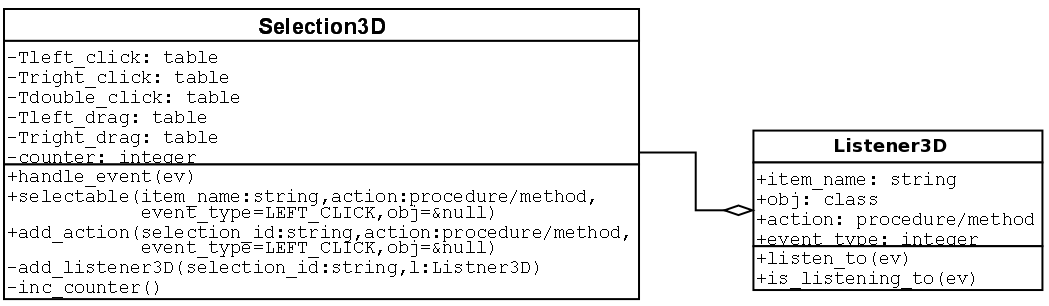
\includegraphics[width=6in,height=1.75in]{utr9/utr9-img035.png}
\end{center}
\begin{center}
\begin{minipage}{5.1264in}
{\selectlanguage{english}
\textbf{Figure 3}. UML diagram for the classes used to manage/control 3D object selection}
\end{minipage}
\end{center}

\bigskip

To make Selection3D class available to a program, the following
statement should be added at beginning of the source code.


\bigskip

{\selectlanguage{english}\sffamily
link Selection3D}


\bigskip

An instance of this class can be created simply by an assignment
statement. The following example line creates this instance and store
it in a variable called \textsf{select3D:}

\bigskip

{\selectlanguage{english}\sffamily
select3D := Selection3D()}


\bigskip

The \textsf{Selection3D} class has three methods that can be called
to manage the 3D selection in the program. The first method is
\textsf{selectable()}, which is used to register new 3D objects to
make them selectable. This method takes up to four parameters in the
following order

\bigskip

\liststyleLix
\begin{enumerate}
\item {\selectlanguage{english}
A string name of the 3D object. The name does not affect the selection behavior in any way. }
\item {\selectlanguage{english}
A procedure/method name to be called when this 3D object is selected}
\item {\selectlanguage{english}
An optional event type which could be any of the event types shown in Figure 2. The default event type is
\textsf{LEFT\_CLICK}}
\item {\selectlanguage{english}
The class object that has the method name (second parameter). This is only valid (and mandatory) if the second
parameter is a method which is part of a class object.}
\end{enumerate}

\bigskip

The method \textsf{selectable()} returns a string value which is
referred to as a selection\_id. A selection\_id is a unique value
that can then be passed to \textsf{WSection()} to mark a new
3D object name. The following is an example of such use

\bigskip

{\selectlanguage{english}\sffamily
select\_id := select3D.selectable({\textquotedbl}red ball{\textquotedbl}, on\_red\_ball)~~ \newline
WSection(select\_id)}

\bigskip

In this example a 3D object named \textsf{{}``red ball''} was
registered to be selectable. The procedure \textsf{on\_red\_ball} will
be called if this 3D object is selected. No event type was passed in
the call so this 3D object will respond to mouse left
click. \textsf{on\_red\_ball} must be a procedure name (not a method)
so nothing should be passed as a fourth parameter also. The example
also shows how is the returned value \textsf{select\_id} was passed to
\textsf{WSection()}.

\bigskip

The second method in Selection3D class is \textsf{add\_action()}. This
method takes four parameters exactly like \textsf{selectable()} except
for the first parameter. Instead of taking a random string name, it
takes a string name that was returned and registered by
\textsf{selectable()} to add another action or response to another
kind of event.  In the example above the following line of code can be
added right after the first line to make the red ball respond to mouse
right click by calling the procedure \textsf{on\_right\_click():}


\bigskip

{\selectlanguage{english}\sffamily
select3D.add\_action(select\_id, on\_right\_click, select3D.RIGHT\_CLICK)~~ \newline
}

The third and the last method in the Selection3D class is
\textsf{handle\_event()}. Normally this method should be part
of the event handling loop in the program. At least all types of mouse
events in Unicon should be passed to this method. This lets the
\textsf{Selection3D} class to collect events information and picked
objects through \textsf{\&pick} and take the appropriate
action. Failure to pass any kind of mouse events to the
\textsf{Selection3D} class might cause it not to produce the interned
behavior. i.e. 3D object selection would not work as you expect. A
correct way to use the method \textsf{handle\_event()} is
shown toward the end of the following complete example

\subsection[]{\color{black} }
{\selectlanguage{english}\sffamily
link selection3D\newline
global select3D\newline
procedure on\_red\_ball()\newline
 write({\textquotedbl} You picked the red ball!{\textquotedbl}) \newline
end}

{\selectlanguage{english}\sffamily
procedure on\_blue\_ball()\newline
 write({\textquotedbl}You picked the blue ball{\textquotedbl})\newline
end\newline
\newline
procedure main()\newline
 \&window := open({\textquotedbl}3D selection in Unicon{\textquotedbl},
{\textquotedbl}gl{\textquotedbl},{\textquotedbl}size=500,500{\textquotedbl}) {\textbar}\newline
\ \  stop({\textquotedbl}can't open 3D window{\textquotedbl}) \newline
 select3D := Selection3D()\newline
 \# begin a new selectable section/object with the name {\textquotedbl}red ball{\textquotedbl}\newline
 WAttrib({\textquotedbl}pick=on{\textquotedbl}) \#turn on 3D selection \newline
 select\_id := select3D.selectable({\textquotedbl}red ball{\textquotedbl}, on\_red\_ball) \newline
 WSection(select\_id)\newline
 \ \ Fg({\textquotedbl}red{\textquotedbl})\newline
 \ \ DrawSphere(1, 0.5, 0, 0.5)\newline
 \ \ WSection() \# end of the red ball \newline
\newline
 \ \ \# Draw a nonselectable green ball\newline
 \ \ Wattrib({\textquotedbl}pick=off{\textquotedbl}) \#turn off 3D selection\newline
 \ \ Fg({\textquotedbl}green{\textquotedbl})\newline
 \ \ DrawSphere(-1, 0.5, 0, 0.5) \newline
\newline
 \ \ \# begin a new selectable section/object with the name {\textquotedbl}blue ball{\textquotedbl} \newline
 \ \ WAttrib({\textquotedbl}pick=on{\textquotedbl}) \#turn on 3D selection\newline
 \ \ select\_id := select3D.selectable({\textquotedbl}blue ball{\textquotedbl}, on\_blue\_ball)\newline
 \ \ WSection(select\_id)\newline
 \ \ \ \ Fg({\textquotedbl}blue{\textquotedbl})\newline
 \ \ \ \ DrawSphere(0, -0.5, 0, 0.5)\newline
 \ \ WSection() \# end of the blue ball \newline
\newline
 \ \ \#setup the eye just to make sure where are looking exactly at the spheres\newline
 \ \ Eye(0,0,4, 0,0,0, 0,1,0)\newline
 \ \ Refresh() \newline
 \ \ repeat\{ \ \ \ \ \ \ \# enter an event loop to handle user events \newline
 \ \ if (ev := {\textbackslash}Event()) then\{\newline
\ \  select3D.handle\_event(ev)\newline
\ \  if ev ===({\textquotedbl}{\textbackslash}e{\textquotedbl}{\textbar}{\textquotedbl}q{\textquotedbl}) then
exit(0)\newline
\ \  \} \newline
 \ \ \ \ \ \}\newline
end}



\section[4. Open Issues and Conclusions]{4. Open Issues and Conclusions}


The Unicon 3D graphics facilities provide many of the features of 3D
graphics programming. Several areas in which improvements and
extensions can be made have been discussed where appropriate in
previous sections. Besides those topics already mentioned throughout
the paper, there are several areas where work could still be
done. These areas include animation, composition, and simplification
of the design of the matrix stack.

The Unicon 3D graphics facilities do not contain special features to
simplify the process of animation. Future work may include the
examination of different ways to directly support animation in Unicon.

Composition is viewing several different pieces as one piece. For
example, say the user wants to implement a moving car.  To do this,
the user would need to break the car into several pieces, possibly,
four tires, a car body, windows, and lights. To make the process of
simulating the moving car easier, one would like these individual
pieces to be one piece. Currently, a Unicon programmer can develop
such applications using the 3D graphics facilities. The question
remains whether composition should be added as a feature of the Unicon
3D graphics facilities.

The design of matrices and transformation in the Unicon 3D graphics
facilities is similar to the design of OpenGL. For this reason, there
is no advantage gained over OpenGL in the area of transformations. It
might be necessary in the future to consider ways to simplify matrices
and transformation in Unicon. One improvement to consider is a
reduction in the number of parameters needed for function like
\textsf{Translate()}, \textsf{Rotate()} and \textsf{Scale()}. The
elimination of the need for two different matrix stacks might be
another simplification.

The current Unicon 3D graphics facilities have made an improvement
over OpenGL in terms of the number of lines of coded needed to
implement a 3D graphics application. Programmers that want to develop
3D graphics applications but do not have the time to learn one of the
standard toolkits might find this project valuable. Although the
Unicon 3D graphics facilities provide the important feature of 3D
graphics, there are some limitations. One limitation might be the lack
of some feature in Unicon that are available in OpenGL. Another
limitation might be the use of default parameters that are used in
some feature of the Unicon 3D graphics facilities. These defaults
reduce the flexibility of the programmer and will be seen as a
restriction by some. Future work on the Unicon 3D graphics facilities
might include the addition of attributes or other mechanisms to remove
those of these limits which prove to be problems. The current Unicon
3D graphics facilities provide a basis in which 3D graphics can be
implemented in Unicon.


\section[5. Functions and Attributes]{5. Functions and Attributes}

The built-in functions attributes in the Unicon 3D graphics facilities
are described in this section. For all functions with a window
argument W, the parameter can be omitted. Also the use of ``{\dots}''
indicates that more arguments can be given. By doing this, the result
is similar to that of multiple function calls. The window argument
should not be specified again for this case.

\bigskip


\subsection[5.1 New Functions]{5.1 New Functions}

The functions in this section have been added specifically for the
Unicon 3D graphics facilities.

\noindent\hrulefill\\
\noindent\textsf{\textbf{DrawCube(file, real, real, real, real,{\dots}): record}} \hfill draws a cube


\bigskip

{\selectlanguage{english}
\textsf{DrawCube(W, x, y, z, l{\dots}) }draws a cube with sides of length l at the position (x, y, z) on the window W.
The display list element is returned. This procedure fails if the context attribute, dim, is set to 2. }


\noindent\hrulefill\\
\noindent\textsf{\textbf{DrawCylinder(file, real, real, real, real,
real, real,{\dots}): record}}\hfill draws a cylinder}


\bigskip

\textsf{DrawCylinder(W, x, y, z, h, r1, r2, {\dots})} draws a
cylinder with a top of radius r1, a bottom with radius r2, and a
height h. The disk is centered at the point (x, y, z). The display
list element is returned. This procedure fails if the context
attribute dim is set to 2.

\noindent\hrulefill\\
\noindent\textsf{\textbf{DrawDisk(file, real, real, real, real, real,
	real, real,\dots): record}}\hfill draws a partial disk


\bigskip

\textsf{DrawDisk(W, x, y, z, r1, r2, a1, a2, {\dots})} draws
a disk on the window W centered at (x, y, z). The inner circle has
radius r1 and the outer circle has radius r2. The parameters a1 and a2
are optional. If they are specified, a partial disk is drawn with a
starting angle a1 and sweeping angle a2. The display list element is
returned.

\noindent\hrulefill\\
\noindent\textsf{\textbf{DrawSphere(file, real, real, real,
real,{\dots}): record}}\hfill draws a sphere

\textsf{DrawSphere(W, x, y, z, r,{\dots})} draws a sphere with
radius r centered at (x, y, z) on the window W. The display list
element is returned. This procedure fails if the context attribute dim
is set to 2.

\noindent\hrulefill\\
\noindent\textsf{\textbf{DrawTorus(file, real, real, real, real, real,{\dots}): record}}
\hfill draw a torus


\bigskip

\textsf{DrawTorus(W, x, y, z, r1, r2,{\dots})} draws a torus with
inner radius r1, outsider radius r2, and centered at (x, y, z) on the
window W. The display list element is returned. This procedure fails
if the context attribute dim is set to 2.

\noindent\hrulefill\\
\noindent\textsf{\textbf{Eye(file, real, real, real, real, real,{\dots}): record}} \hfill place camera


\bigskip

\textsf{Eye(W, x, y, z, x2, y2, z2, x3,y3,z3)} places the camera at
position (x1,y1,z1) looking at the point (x2,y2,z2). The direction
(x3,y3,z3) will be ``up'' in the rendered scene.

\noindent\hrulefill\\
\noindent\textsf{\textbf{IdentityMatrix(file): record}}
\hfill load the identity matrix


\bigskip

\textsf{IdentityMatrix(W)} changes the current matrix to the identity
matrix. The display list element is returned.


\bigskip

\noindent\hrulefill\\
\noindent\textsf{\textbf{MatrixMode(file, string): record}}
\hfill changes the matrix mode


\bigskip

\textsf{MatrixMode(W, s)} changes the matrix mode to s. The string s
must be either \textsf{{}``projection''} or \textsf{{}``modelview''},
otherwise this procedure fails. The display list element is returned.


\bigskip

\noindent\hrulefill\\
\noindent\textsf{\textbf{MulMatrix(file, x): list}}
\hfill multiply transformation matrix


\bigskip

\textsf{MulMatrix(W, L)} multiply transformation matrix by the list L
where *L is 16.

{\selectlanguage{english}
\textsf{MulMatrix(W, x}\textsf{\textsubscript{1}}\textsf{, {\dots}, x}\textsf{\textsubscript{16}}\textsf{) }multiply
transformation matrix by the numbers x\textsubscript{1} ... x\textsubscript{16.}}

In both cases above, the values represent a matrix of size 4x4 stored
in column format. The values should be {\em exactly\/} 16
otherwise the function will fail.

\noindent\hrulefill\\
\noindent\textsf{\textbf{Normals(file, x): list}}\hfill set normals

\textsf{Normals(W, L)} sets the normals to use for subsequent
rendered objects to those given in list L.

\textsf{Normals(W, x\textsubscript{1},y\textsubscript{1},z\textsubscript{1}, ..., x\textsubscript{n},y\textsubscript{n}, z\textsubscript{n})}
sets the normals to use for subsequent rendered objects to x, y and z
values. Each x, y, z triple forms one normal coordinate that corresponds
to one vertex.

In all cases the display list element is returned.

\noindent\hrulefill\\
\noindent\textsf{\textbf{PopMatrix(file): record}}
\hfill pop a matrix from the matrix stack


\bigskip

\textsf{PopMatrix(W)} pops the top matrix from the matrix stack. The matrix stack is determined by the current matrix
mode, either \textsf{{}``projection''} or \textsf{{}``modelview''.} This procedure fails if there is only one matrix on
the matrix stack. The display list element is returned.

\noindent\hrulefill\\
\noindent\textsf{\textbf{PushMatrix(file): record}}
\hfill push a matrix onto the matrix stack


\bigskip

\textsf{PushMatrix(W)} pushes a copy of the current matrix onto the
matrix stack. The current matrix mode determines what stack the new
matrix is pushed upon. This procedure fails if the matrix mode is
\textsf{{}``projection''} and there are already two matrices on the
stack. If the matrix mode is \textsf{{}``modelview''} and there are
already thirty two matrices on the stack, then this procedure will
fail. The display list element is returned.

\noindent\hrulefill\\
\noindent\textsf{\textbf{Refresh(file):file}} \hfill redraw the window


\bigskip

\textsf{Refresh(W)} redraws the contents of the window.
The window W is returned.

\noindent\hrulefill\\
\noindent\textsf{\textbf{Rotate(file, real, real, real, real,{\dots}): record}}
\hfill rotate objects


\bigskip

{\selectlanguage{english}
\textsf{Rotate(W, a, x, y, z,{\dots})} rotates objects affected by this transformation by the angle a, in around the
axis represented by the vector formed of the (x, y, z) values. The display list element is returned.}

\noindent\hrulefill\\
\noindent\textsf{\textbf{Scale(file, real, real, real,{\dots}): record}} \hfill
scales objects


\bigskip

\textsf{Scale(W, x, y, z,{\dots})} scales object according to the
given x, y and z coordinates. The display list element is returned.

\noindent\hrulefill\\
\noindent\textsf{\textbf{Texcoord(file, X):list}}
\hfill define texture coordinates


\bigskip

\textsf{Texcoord(W, x}\textsf{\textsubscript{1}}\textsf{, y}\textsf{\textsubscript{1}}\textsf{, {\dots},
x}\textsf{\textsubscript{n}}\textsf{, y}\textsf{\textsubscript{n}}\textsf{) }sets the texture coordinates to
\textsf{x}\textsf{\textsubscript{1}}\textsf{, y}\textsf{\textsubscript{1}}\textsf{, {\dots},
x}\textsf{\textsubscript{n}}\textsf{, y}\textsf{\textsubscript{n}}\texttt{\textsubscript{. }}Each x, y, pair forms one
texture coordinate. Every x must match to a y otherwise the assignment of texture coordinates will fail.

\textsf{Texcoord(W, L)} sets the texture coordinates to those specified in the list \textsf{L}.

\textsf{Texcoord(W, s) }sets the texture coordinates to those
specified by \textsf{s}. The string \textsf{s} must be
\textsf{{}``auto''} otherwise the procedure will fail. In all cases
the display list element is returned.

\noindent\hrulefill\\
\noindent\textsf{\textbf{Texture(file, X): record}} \hfill apply a texture


\bigskip

\textsf{Texture(W, s) }creates a texture image that is applied to
subsequent objects on the window \textsf{W}. The string \textsf{s}
specifies the texture image as a filename, a string of the form
\textsf{width,pallet,data} or \textsf{width,\#,data}, where pallet is
a pallet from the Unicon 2D graphics facilities and data is the
hexadecimal representation of an image. The display list element is
returned.

\textsf{Texture(W1, W2) }creates a texture image that is applied to
subsequent objects on the window \textsf{W1}. The file \textsf{W2} is
another Unicon window. The contents of \textsf{W2} are used to create
the texture image. The display list element on \textsf{W1} is
returned.

\textsf{Texture(W1, R) }creates a texture image that is applied to
subsequent objects on the window \textsf{W1}. The Record \textsf{R} is
another texture record that will be used to create the new texture
reusing R texture data. This is useful to reapply the same texture on
different places in the program.

\noindent\hrulefill\\
\noindent\textsf{\textbf{Translate(file, real, real, real,{\dots}): record}}
\hfill translate objects


\bigskip

{\selectlanguage{english}
\textsf{Translate(W, x, y, z,{\dots})} moves objects affected by this transformation in the direction (x, y, z). The
display list element is returned.}

\noindent\hrulefill\\
\noindent\textsf{\textbf{WindowContents(file):list}}
\hfill produce contents of window


\bigskip

\textsf{WindowContents(W)} returns a Unicon list of display elements,
which are records or lists. Each element has a function name followed
by the parameters of the function, or an attribute followed by its
value. The display list is further described in section 3.6.

\bigskip

\bigskip

\subsection[5.2 Extensions from the 2D Graphics Facilities]
{5.2 Extensions from the 2D Graphics Facilities}


\bigskip

Several functions from the Unicon 2D graphics facilities have been
modified for use in the 3D facilities. This section describes the
parameters and use of these functions.

\bigskip

\bigskip

\noindent\hrulefill\\
\noindent\textsf{\textbf{DrawLine(file, real, real, real, {\dots}): list}}
\hfill draw a line


\bigskip

\textsf{DrawLine(W, x1, y1, z1, {\dots},xn, yn, zn)} draws a line
connecting the n vertices specified by (x, y, z). If only one set of
vertices is given, then no line is drawn. If the attribute
\textsf{dim} is set to 2, then
\textsf{DrawLine(W, x1, y1,{\dots},xn, yn)}
draws a line connecting the n vertices of the form (x, y). If
the attribute \textsf{dim} is set to 4, then

\textsf{DrawLine(W, x1, y1,z1, w1{\dots},xn, yn,zn, wn)}
draws a line connecting the n vertices of the form (x, y, z, w).
The display list element is returned.


\bigskip

DrawLine(W, L) draws lines whose coordinates are passed as a list of
real values.

\noindent\hrulefill\\
\noindent\textsf{\textbf{DrawPoint(file, real, real, real, {\dots}): list}}
\hfill draw points


\bigskip

\textsf{DrawPoint(W, x1, y1, z1, {\dots})} for each set of vertices
(x, y, z) a point is drawn. If the attribute \textsf{dim} is set to 2,
then \textsf{DrawPoint(W, x1, y1,{\dots})}\texttt{ }draws points of
the form (x, y). If the attribute \textsf{dim} is set to 4, then
\textsf{DrawPoint(W, x1,y1,z1,w1{\dots}) }draws points of the form (x,
y, z, w). The display list element is returned.


\bigskip

DrawPoint(W, L) draws points whose coordinates are passed as a list of
real values.

\noindent\hrulefill\\
\noindent\textsf{\textbf{DrawPolygon(file, real, real, real, {\dots}): list}}
\hfill draw a polygon


\bigskip

\textsf{DrawPolygon(W, x1, y1, z1, {\dots}, xn, yn, zn)} draws an
outline of a polygon formed by connecting the n vertices of the form
(x, y, z). If the value of the context attribute \textsf{dim} is 2
then \textsf{DrawPolygon(W, x1, y1, {\dots}, xn, yn)} draws an outline
of a polygon using the n vertices of the form (x, y). If
\textsf{dim} is set to 4, then \textsf{DrawPolygon(W, x1, y1, z1, w1
{\dots}, xn, yn, zn, wn)} draws an outline of a polygon formed by
connecting the n vertices of the form (x, y, z, w). The display list
element is returned.

DrawPolygon(W, L) draws polygons/shapes whose coordinates are passed
as a list of real values.


\bigskip

This function can be used to draw shapes other than polygons, this
feature can be controlled by the attribute \textsf{meshmode} which is
discussed in the New Attributes section.

\noindent\hrulefill\\
\noindent\textsf{\textbf{DrawSegment(file, real, real, real, {\dots}): list}}
\hfill draw segments


\bigskip

\textsf{DrawSegment(W, x1, y1, z1, x2, y2, z2,{\dots})} draws a line
segment between a pair of vertices of the form (x, y, z). If the
context attribute \textsf{dim} has value 2 then
\textsf{DrawSegment(W, x1, y1, x2, y2,{\dots})}
draws a line segment between a pair of
vertices of the form (x, y). If the context attribute \textsf{dim} has
value 4 then
\textsf{DrawSegment(W, x1, y1, z1, w1, x2, y2, z2, w2,{\dots})}
draws a line segment between a pair of vertices of the
form (x, y, z, w). If an odd number of vertices if given, then the
last vertex is ignored. The display list element is returned.


\bigskip

DrawSegment(W, L) draws line segments whose coordinates are passed
as a list of real values.


\bigskip

\noindent\hrulefill\\
\noindent\textsf{\textbf{EraseArea():file}} \hfill clear the contents of the window


\bigskip

\textsf{EraseArea(W)} clears the contents of the window. Although the 2D facilities allow for specifying a specific
area, \textsf{EraseArea()} erases the entire contents of a 3D window.

\noindent\hrulefill\\
\noindent\textsf{\textbf{Fg(file, string):string}} \hfill get/set foreground color


\bigskip

\textsf{Fg(W, s)} changes the material properties of subsequently
drawn objects to the material properties specified by s. The string s
must be one or more semi-colon separated material properties. A
material property is of the form

$\left[
\begin{array}{l}
diffuse\\ambient\\specular\\emission
\end{array}
\right]$ \textsf{\textit{color name}} or \textsf{``shininess n''},
where \textsf{n} is between \textsf{0} and \textsf{128}.

If string s is omitted, the current values of the material properties
will be returned.


\noindent\hrulefill\\
\noindent\textsf{\textbf{FillPolygon(file, real, real, real, {\dots}): list}}
\hfill draw a filled polygon


\bigskip

\textsf{FillPolygon(W, x1, y1, z1, {\dots}, xn, yn, zn)} draws a
filled polygon formed from the n vertices of the form (x, y, z) and
the current foreground color. If the context attribute \textsf{dim} is
set to 2, then \textsf{FillPolygon(W, x1, y1, {\dots}, xn, yn)} draws
a filled polygon formed from the n vertices of the form (x, y) and the
current foreground color. If \textsf{dim} is set to 4, then
\textsf{FillPolygon(W, x1, y1, z1, w1 {\dots}, xn, yn, zn, wn)} draws
a filled polygon formed from the n vertices of the form (x, y, z, w)
and the current foreground color. The display list element is
returned.

FillPolygon(W, L) draws filled polygons/shapes whose coordinates
are passed as a list of real values.


\bigskip

This function can be used to draw shapes other than polygons, this
feature can be controlled by the attribute
\textsf{meshmode} which is discussed in the New Attributes section.


\bigskip

\subsection[5.3 New Attributes]{5.3 New Attributes}


\bigskip

This section describes the new context attributes that have been
added specifically for the 3D graphics facilities.


\bigskip

\noindent\hrulefill\\
\noindent\textsf{\textbf{dim}} \hfill dimensionality of graphic objects

\bigskip

The functions
\textsf{DrawLine(), DrawPolygon(), DrawSegment(), DrawPoint(),}
and \textsf{FillPolygon(),} use the value of
\textsf{dim} to determine how many coordinates each vertex has. If
\textsf{{}``dim = 2''} then
\textsf{DrawTorus(), DrawSphere(), DrawCube()}, and
\textsf{DrawCylinder()} cannot be used.


\bigskip

Values: \textsf{{}``2''}, \textsf{{}``3''}, or \textsf{{}``4''}

Default value: \textsf{{}``3''}

\noindent\hrulefill\\
\noindent\textsf{\textbf{eye}} \hfill point of view


\bigskip

This attribute assigns the eyepos, eyedir, and eyeup attributes.
See also the \textsf{Eye()} function.


\bigskip

Default value: \ \textsf{{}``(0.0, 0.0, 0.0, 0.0, 0.0, 0.0, 0.0, 1.0, 0.0)''}

\noindent\hrulefill\\
\noindent\textsf{\textbf{eyedir}} \hfill eye direction


\bigskip

The eye direction is the direction in which the eye is looking.


\bigskip

Default value: \ \textsf{{}``(0.0, 0.0, 0.0)''}

\noindent\hrulefill\\
\noindent\textsf{\textbf{eyepos}} \hfill eye position


\bigskip

The eye position is the where the eye is currently located.


\bigskip

Default value: \ \textsf{{}``(0.0, 0.0, 0.0)''}

\noindent\hrulefill\\
\noindent\textsf{\textbf{eyeup}} \hfill up direction


\bigskip

The eyeup attribute specifies what direction is up in the scene.


\bigskip

Default value: \ \textsf{{}``(0.0, 1.0, 0.0)''}

\noindent\hrulefill\\
\noindent\textsf{\textbf{glrenderer}} \hfill 3D renderer


\bigskip

Read only attribute that gives the specific hardware configuration
(video card name) that is used to render 3D graphics.

\noindent\hrulefill\\
\noindent\textsf{\textbf{glvendor}} \hfill 3D vendor


\bigskip

Read only attribute that gives the vendor of the 3D graphics
library implementation.

\noindent\hrulefill\\
\noindent\textsf{\textbf{glversion}} \hfill 3D version


\bigskip

Read only attribute that gives the 3D graphics library version number.


\bigskip

\noindent\hrulefill\\
\noindent\textsf{\textbf{light0...light7}} \hfill light source properties


\bigskip

There are eight lights in the Unicon 3D graphics facilities. Each
light can be assigned values to each of its properties on/off,
diffuse, ambient, specular, and position. The values of diffuse,
ambient, specular are a color specification.  The position is given by
a (x, y, z) coordinate. The default values are as follows for the
lights.


\bigskip


\bigskip

\begin{center}
\tablefirsthead{}
\tablehead{}
\tabletail{}
\tablelasttail{}
\begin{supertabular}{|m{0.56295985in}|m{0.5775598in}|m{1.1288599in}|m{1.2427598in}|m{1.0427599in}|m{0.9754599in}|}
\hline
\centering{\selectlanguage{english} Light} &
\centering{\selectlanguage{english} On/Off} &
\centering{\selectlanguage{english} Diffuse} &
\centering{\selectlanguage{english} Ambient} &
\centering{\selectlanguage{english} Specular} &
\centering\arraybslash{\selectlanguage{english} Position}\\\hline
{\selectlanguage{english} \textsf{\textbf{light0}} } &
\centering{\selectlanguage{english} On} &
\centering{\selectlanguage{english} white} &
\centering{\selectlanguage{english} black} &
\centering{\selectlanguage{english} white} &
\centering\arraybslash{\selectlanguage{english} (0.0, 0.0, 1.0)}\\\hline
{\selectlanguage{english}\sffamily\bfseries light1- light7} &
\centering{\selectlanguage{english} Off} &
\centering{\selectlanguage{english} black} &
\centering{\selectlanguage{english} black} &
\centering{\selectlanguage{english} black} &
\centering\arraybslash{\selectlanguage{english} (0.0,0.0,1.0)}\\\hline
\end{supertabular}
\end{center}

\bigskip

\noindent\hrulefill\\
\noindent\textsf{\textbf{texcoord}} \hfill texture coordinates


\bigskip

The attribute \textsf{texcoord} can be assigned the value \textsf{{}``auto'',} or a string of texture coordinates. If
\textsf{texcoord} has the value \textsf{{}``auto'',} texture coordinates are determined by the Unicon 3D graphics
facilities. Otherwise texture coordinates, which are pairs (x, y) with x and y are between 0.0 and 1.0, are obtained
from attribute \textsf{texture}.


\bigskip

Default:\ \ \textsf{{}``auto''}.

\noindent\hrulefill\\
\noindent\textsf{\textbf{meshmode}} \hfill mesh mode type


\bigskip

The \textsf{meshmode} attribute changes how the coordinates passed to
\textsf{DrawPolygon()} and \textsf{FillPolygon()} will be interpreted.
This attribute can take the following values: \textsf{{}``points''},
\textsf{{}``lines''}, \textsf{{}``linestrip''}, \textsf{{}``lineloop''},
\textsf{{}``triangles''}, \textsf{{}``trianglefan''},
\textsf{{}``trianglestrip''}, \textsf{{}``quads''},
\textsf{{}``quadstrip''} and \textsf{{}``polygon''}.


\bigskip

Default:\ \ \textsf{{}``polygon''}.


\bigskip

\noindent\hrulefill\\
\noindent\textsf{\textbf{normode}} \hfill enable/disable normals


\bigskip

If normode has the value \textsf{{}``auto''}, then normals are
automatically generated for each drawn polygon so that the normal is
perpendicular on the polygon and pointing away from it. If normode has
the value of ``on'' then the user can supply custom normals using the
\textsf{Normals()} function. Otherwise normode has the value
\textsf{{}``off''}, which indicates objects are drawn using a default
preset normal. By default normode has the value \textsf{{}``auto''.}

\noindent\hrulefill\\
\noindent\textsf{\textbf{rings}} \hfill sets the number of rings


\bigskip

rings should be an integer value greater than 0. It controls the level
of details for drawing spheres, cylinders and toruses by setting the
number of rings used to draw those objects. By default slices has the
value 15.


\bigskip

\noindent\hrulefill\\
\noindent\textsf{\textbf{slices}} \hfill sets the number of slices


\bigskip

slices should be an integer value greater than 0. It controls the
level of details for drawing spheres, cylinders, toruses and disks by
setting the number of slices used to draw those objects. By default
slices has the value 15.


\bigskip

\noindent\hrulefill\\
\noindent\textsf{\textbf{texmode}} \hfill enable/disable texturing


\bigskip

If texmode has the value \textsf{{}``on'',} then textures are mapped
onto drawn objects. Otherwise texmode has the value
\textsf{{}``off''}, which indicates objects are drawn using the
background color. By default texmode has the value \textsf{{}``off''.}

\noindent\hrulefill\\
\noindent\textsf{\textbf{texture}} \hfill texture image


\bigskip

\noindent
The attribute texture is assigned a filename or a string of the
following format.

\texttt{\ \ \ }\textsf{width,pallet,data} \ or \ \ \textsf{width,\#,data}

\noindent
where \textsf{pallet} is a pallet defined in the Unicon 2D graphics
facilities and data is the hexadecimal representation of an image.
The value assigned to texture is used to create a texture image
which is applied to subsequent objects on the window.


\subsection[5.4 Extensions from the 2D Graphics Attributes]
{5.4 Extensions from the 2D Graphics Attributes}


\bigskip

Several attributes have been extended to be used in the 3D graphics
facilities. The new meanings of these attributes are described in
this section.


\bigskip

\noindent\hrulefill\\
\noindent\textsf{\textbf{fg}} \hfill foreground color and material properties


\bigskip

The string assigned to fg must be one or more semi-colon
material properties. A material property is of the form

$\left[
\begin{array}{l}
diffuse\\ambient\\specular\\emission
\end{array}
\right]$ \textsf{\textit{color name}} or \textsf{``shininess n''},
where \textsf{n} is between \textsf{0} and \textsf{128}.


\noindent\hrulefill\\
\noindent\textsf{\textbf{linewidth}} \hfill width of lines

\bigskip

\noindent
The line width in 3D windows is a real number in world coordinates.

\bigskip

\noindent
Default value: \texttt{1.0}


\section[References]{References}


\noindent
[Foley82]\ \ Foley, J.D; and A.Van Dam.
Fundamentals of Interactive Computer Graphics. Reading, MA: Addison-Wesley
Publishing Company, 1982.


\bigskip

\noindent
[Griswold96] \ \ Griswold, Ralph E and Griswold, Madge T.
The Icon Programming Language, Third Edition. San Jose, CA:
Peer-To-Peer Communications, 1996.

\bigskip

\noindent
[Griswold98]\ \ Griswold, Ralph E.; Jeffery, Clinton L.; and Townsend, Gregg M.
Graphics Programming in Icon. San Jose, CA.
Peer-To-Peer Communications, 1998.

\bigskip

\noindent
[Jeffery03]\ \ Jeffery, Clinton; Mohamed, Shamim; Pereda, Ray; and
Parlett, Robert. Programming with Unicon. Open book published from
http://unicon.org


\bigskip

\noindent
[JeffMart03]\ \ Jeffery, Clinton and Martinez, Naomi.
The Implementation of Graphics in Unicon Version 11. Unicon
Technical Report \#5a, \href{http://unicon.org/}{http://unicon.org}, 2003.

\bigskip

\noindent
[OpenGL99] \ \ OpenGL Architecture Review Board;
Woo, Mason; Neider, Jackie; Davis, Tom; Shreiner, Dave.
OpenGL Programming Guide: the Official Guide to
Learning OpenGL, Third Edition. Reading, MA: Addison-Wesley
Publishing Company, 1999.


\bigskip

\noindent
[OpenGL00] \ \ OpenGL Architecture Review Board; Shreiner, Dave.
OpenGL Programming Guide: the Official Reference Document to
OpenGL, Third Edition. Upper Saddle Reading, MA: Addison-Wesley
Publishing Company, 2000.


\bigskip

\noindent
[Walker94]\ \ Walker, Kenneth; The Run-Time Implementation Language
for Icon. Technical Report from http://www.cs.arizona.edu/icon/

\end{document}
